\documentclass[12pt,letterpaper,spanish,openright]{report}
\usepackage[activeacute,spanish,mexico]{babel}
\usepackage[dvips]{graphicx}
\usepackage{amsmath}
\usepackage[latin1]{inputenc} 
\usepackage[absolute]{textpos}
\usepackage{multirow, array}
\usepackage{float}
\usepackage{setspace}
\oddsidemargin 0cm \headsep 0.5cm
\textwidth=16cm \textheight=20cm
\usepackage{eso-pic}
\usepackage[hidelinks]{hyperref}
\usepackage{url}
\usepackage{pgfgantt}
\usepackage{verbatim}
\usepackage[dvips]{graphicx}
\DeclareGraphicsExtensions{.bmp,.png,.pdf,.jpg}

\usepackage{multicol}
\usepackage{wrapfig}
\usepackage{subfigure}
\usepackage{enumerate} 
\usepackage{listings}
\graphicspath{{img/}}

\begin{document}
\begin{titlepage}
\begin{figure}
\centering

\includegraphics[scale=0.75]{upj.png}
\end{figure}

\begin{center}
\huge{UNIVERSIDAD POLIT�CNICA DE JUVENTINO ROSAS}\\

\vspace{1.0cm}

\large{\textbf{Proyecto Integrador}}
\vspace{1.0cm}



{ \large \bfseries ``Tech-Tuin''  \\[0.4cm] }


\vspace{1.0cm}

%{QUE PARA OBTENER EL T�TULO DE \\\textbf{INGENIERO EN TELEM�TICA}}

\vspace{1.0cm}


\emph{Presenta:}\\
Aide \textsc{Pizano Escalante}\\
Cristian Iv�n \textsc{Mu�iz Mnedoza}\\
El�as Abraham	\textsc{Ramirez Rivera}\\
Jos� Martin	\textsc{Nieto Le�n}\\
V�ctor Alfonso	\textsc{Humareda Barbosa}\\

\emph{Asesores:} \\
M.I. Luis Rey Lara Gonz�lez

\vspace{1.5cm}

\noindent{Santa Cruz de Juventino Rosas, Gto. 13 de Agosto de 2018.}
\end{center}

\end{titlepage}
%\chapter*{Agradecimientos}
\pagenumbering{Roman} % para comenzar la numeracion de paginas en numeros romanos

\textit{Primeramente, le agradezco a Dios, pues me ha dado la vida, la inteligencia, la fuerza y la determinaci\'on para cumplir mis metas y prop\'ositos. De la misma manera agradezco a mi padre V\'ictor Manuel Cruz Hern�ndez y mi madre Rosa Mar\'ia Casta�eda Castillo en quienes siempre encuentro amor y apoyo para seguir adelante, porque gracias a su esfuerzo y sacrificio he llegado hasta donde estoy, a ellos les debo mi carrera, mi vida y mis triunfos. Le agradezco a mi hermana Mayela Montserrat porque tengo la certeza de que cuando la necesite siempre estar\'a a mi lado para apoyarme. Agradezco tambi\'en a mis t\'ios Teresa Casta�eda y Edie Haro por su hospitalidad y apoyo durante el seguimiento de mi Estad\'ia Del mismo modo le agradezco a mis amigos y compa�eros de Santa Cruz de Juventino Rosas que fueron y son parte de mi vida, al Profesor Carlos Aguado qui\'en desde el primer momento confi\'o en mi ciegamente sin a\'un conocerme, le agradezco infinitamente su hospitalidad, sus consejos y sobre todo su apoyo desinteresado tambi\'en agradezco a mis amigos Lupita, Beto y Cristian con los que viv\'i durante 3 a�os y compart\'i muchos momentos agradables, no pueden faltar mis amigos y compa�eros de generaci\'on, a todos ustedes muchas gracias, siempre me han ayudado a levantarme cuando he ca\'ido y siguen a mi lado cuando los necesite, s\'e que nuestra amistad se mantendr\'a por muchos a�os.
Le agradezco a mi tutor el M.I. Jos\'e Gabriel Aguilera Gonz\'alez por su apoyo, su dedicaci\'on, compromiso y \'animo durante mi carrera, por el conocimiento que me comparti\'o como profesor adem\'as al estar al frente de la carrera nos motiv\'o y realiz\'o muchas buenas acciones a favor de la misma. De igual modo le agradezco a mis maestros, por guiarme, por sus ense�anzas y el conocimiento compartido, le agradezco a mi asesor M.C. Jos\'e Cristian Padilla Navarro por su motivaci\'on, su paciencia, consejos y apoyo que fue fundamental para mi desarrollo como profesionista. M\'as que maestros algunos fueron amigos que nos guiaban por la carrera, superando obst\'aculos y adversidades. A todos y cada uno de mis profesores gracias. 
}

%\chapter*{Dedicatoria}
\begin{flushright}
\textit{Dedicado a\\
A Dios, y a mis padres.\\
A Dios porque ha estado conmigo a cada paso que doy, \\
cuid\'andome y d\'andome fortaleza para continuar.\\
A mis padres, quienes han sido la gu\'ia y el camino\\
para poder llegar a este punto de mi carrera\\ 
y quienes han velado por mi bienestar y educaci\'on\\ 
siendo mi apoyo en todo momento,\\ 
depositando su confianza en m\'i\\ 
sin dudar ni un solo momento en mi inteligencia y capacidad,\\ 
que con su ejemplo, dedicaci\'on y palabras de aliento\\ 
nunca bajaron los brazos para que yo tampoco lo hiciera\\ 
aun cuando todo se complicaba.\\
Es por ellos que soy lo que soy ahora.\\
A ustedes, con amor.}
\end{flushright}
\chapter*{Resumen} % si no queremos que añada la palabra "Capitulo"
\markboth{RESUMEN}{RESUMEN} % encabezado 
 
Este proyecto consiste en la desarrollo de un sistema de riego automatizado que, en base a un circuito el�ctrico, sea capaz de tomar decisiones tomando en cuenta las condiciones ambientales en tiempo real. El objetivo del proyecto, es reducir el consumo de agua al momento de regar jardines.\\
 Para dise�ar el sistema se investigaron las necesidades del mercado local. Dichas necesidades fueron obtenidas en base a encuestas en l�nea, informes y publicaciones, realizados respectivamente por los miembros del equipo, organizaciones pertinentes y universidades
especializadas.\\
Analizando la informaci�n recabada, se determin� que el principal foco del sistema fuera el riego de �rboles en jardines dom�sticos y que las condiciones ambientales que m�s influyen en el consumo de agua por parte de las plantas son la temperatura del agua, la cantidad suministrada de agua, la humedad del suelo y el momento del d�a en que se riega la planta.\\

\vspace{2.5cm}
\textbf{Palabras clave:} jardin, sistema de riego, automatizaci�n.
\chapter*{Abstract} % si no queremos que añada la palabra "Capitulo"
\markboth{ABSTRACT}{ABSTRACT} % encabezado 
 
This project consists of the development of an automated irrigation system that, based on an electrical circuit, is capable to make decisions taking into consideration the environmental conditions in real-time. The objective of the project, it is to reduce water consumption at the moment of watering gardens.\\
To design the system, the needs of the local market were investigated. These requirements were obtained on the basis of online surveys, reports and publications, conducted respectively by team members, relevant organizations and specialized universities.\\
Analyzing the information collected, it was determined that the main focus of the system was the irrigation of trees in domestic gardens and that the environmental conditions that most in uence the water consumption by the plants are the water temperature, the quantity supplied with water, soil moisture and the time of day the plant is irrigated.

\vspace{2.5cm}
\textbf{Key words:} garden, irrigation system, automation.
\newpage
\begin{doublespace}
\tableofcontents
\cleardoublepage
\addcontentsline{toc}{chapter}{�ndice de figuras} 
\listoffigures 

%\cleardoublepage
%\addcontentsline{toc}{chapter}{�ndice de tablas}
%\listoftables

\chapter{Introducci�n}
\pagenumbering{arabic} 

\section{Definici�n del problema}
D�cada a d�cada la cantidad de agua potable en M�xico se ve disminuida debido al desperdicio inconsciente de la misma. Tan solo en Guanajuato, un habitante promedio consume al rededor de 87 litros al dia., siendo aproximadamente 50\% no reutilizable.
Entre las actividades donde se presenta un mayor consumo de agua se encuentra el riego de jardines dom�sticos por lo que, la implementaci�n de un sistema de riego automatizado ayuda a dar un uso m�s racional del agua, logrando en el proceso una mejora en la condici�n del jard�n.

\newpage
\section{Objetivos}
\subsection{Objetivo General}
Desarrollar e implementar un sistema de riego autom�tico que reduzca el consumo agua al momento de regar jardines dom�sticos, utilizando un circuito electr�nico que sea capaz de tomar decisiones basado en las condiciones ambientales del jard�n.
\subsection{Objetivos espec�ficos}
\begin{itemize}
	\item Elaborar un circuito electr�nico que implemente los sensores necesarios para monitorear	el ambiente.
	\item Dise�ar un circuito el�ctrico en el que se implemente los sensores necesarios para el monitoreo del jard�n.
\end{itemize}

%\chapter{Estado del arte}
%En el estado del arte se hace una revisi�n profunda de los trabajos relacionados con el desarrollo de tu proyecto, de manera que se resalte la contribuci�n que har�s con tu trabajo.

Deber�s incluir al menos $10$ art�culos o revistas, puedes consultar la p�gina del CONRICYT

Ejemplo de cita \cite{BAURA2004}.

\chapter{Estado del Arte}
En (Tejada, 2013) encontramos un proyecto de riego autom�tico y aut�nomo para administrar riego por goteo en peque�os jardines y balcones. Es sistema utiliza un Arduino Uno que se encarga de obtener datos del ambiente y procesarlos para activar un mecanismo de distribuci�n de agua cuando se cumplan una serie de condiciones\cite{1}.\\

En (Gil-Albert, 2006) se describe de manera detallada las especies de pastos que existen, las caracter�sticas de los mismos y los cuidados que requieren. Tambi�n encontramos informaci�n y caracter�sticas de otras plantas de jardines\cite{2}.\\

En (Torrecilla, 1998) encontramos un sistema de riego inteligente mediante una aplicaci�n en donde se decriben los diferentes tipos de suelos para jardines, ademas de sus caracteristicas, componentes y consideraciones a tener en cuenta al momento de sembrar
y cuidar plantas\cite{4}.\\

En(Rios,2016) el documento recoge el dise�o del hardware y software de un programador de riego completo, econ�mico y f�cil de utilizar. A partir de un microcontrolador y tratando las se�ales provenientes de sensores anal�gicos de humedad, luminosidad y temperatura y de un detector de lluvia digital, se controlar�an cinco electrov�lvulas que ser�an activadas y desactivadas en un tiempo determinado y cuando se den las caracter�sticas que desee el usuario\cite{5}.\\

En(Escamilla,2016) la elaboraci�n de este tranajo sugiere de la necesidad de plantear soluciones, para optimizar el uso de agua para regado hortofruticolas, considerando que es tambi�n una herramienta util para el aprovechamiento de los recursos hidricos y con
ello aumentar los niveles de producci�n y de calidad obtenitendo mediante estas tecnicas.
Este trabajo tambien se introduce en el mundo de los microprocesadores, tratando conceptos de electronica, programaci�n y transmision de se�ales\cite{6}.\\

En (Escalas,2015) En este proyecto se propone automatizar los sistemas de riego que instala una empresa de jardiner�a. Para ello se va a crear una plataforma que va a permitir al usuario ver los datos meteorol�gicos y tener un control total sobre su sistema de riego.
Este sistema engloba una serie de sensores conectados a un micro-controlador, a su vez controlado por un micro-procesador con salida a internet, lo que permitir�a controlar la aplicaci�n a distancia. Tanto los sensores como los dos dispositivos son de bajo coste\cite{7}.\\

En (Tarjuelo, 2010) se presenta un proyecto el cual consiste en un sistema de riego en el que se implementan tecnolog�as con el prop�sito de conseguir una id�nea utilizaci�n del agua. Este sistema de riego tiene como objetivo suministrar a las plantas agua de forma eficiente y sin alterar la fertilidad del suelo, as� como interrelacionar los principales componentes de un sistema de riego los cuales son: energ�a, agua, mano de obra y sistematizaci�n\cite{8}.\\

En ( �guila, 2008) se presenta un sistema de riego automatizado en tiempo real con balance h�drico y medici�n de humedad del suelo. Este sistema se enfoca principalmente en el monitoreo por medio de tecnolog�a para determinar el momento oportuno y cantidad de riego de un cultivo o de una planta\cite{9}.\\

En(S�ez, 2017) nos habla sobre un sistema de riego inteligente el cual optimiza el consumo de agua de los cultivos y de jardines, la principal actividad de este sistema es proporcionar una estrategia de distribuci�n para minimizar el consumo total de agua suministrado a cada l�nea de riego bas�ndose en datos obtenidos de cada planta\cite{10}.\\





\chapter{Estudio de Mercado}
El desarrollo del cap�tulo abarca la presentaci�n de conceptos vinculados al estudio de mercado as� como los resultados de una encuesta aplicada sobre la factibilidad del sistema de riego.
\section{An�lisis de la demanda}

En la actualidad, M�xico se encuentra entre los cinco pa�ses que m�s agua consume por habitante en el mundo compartiendo lugar con EU, Australia, Italia y Jap�n. Esto a su vez, convierte a M�xico en uno de los lugares del mundo con m�s baja disponibilidad de agua potable.
Se debe tomar en cuenta que del consumo total de agua potable en el pa�s, el riego representa aproximadamente 66\% del total de extracciones, los hogares el 10\% y la industria
otro 20 \%. Profundizando en el consumo de agua dedicado al riego, el c�sped en jardines domesticas
7
requiere en promedio, entre 7 a 9 litros de agua a la semana.


\subsection{Competidores en el mercado}
En el mercado tenemos varios tipos de sistemas de riego automaticos sin embargo, solo unos cuantos son nuestra competencia, entre ellos estan:
\begin{itemize}
	\item \textbf{Tevatronic}: Esta empresa dise�� un sistema de riego aut�nomo. El sistema Exilong consta de sensores inal�mbricos con controladores de riego en el suelo, y un software que los dirige. Los sensores son enterrados en diferentes �reas del jard�n, y pueden detectar la longitud de la ra�z, la hidrataci�n del suelo, y el consumo de agua.
	Estos sensores transmiten los datos a un controlador de riego. Los controladores de riego se conectan a un enchufe regular de corriente, y pueden controlar hasta cuatro	v�lvulas o zonas de agua. Todos los datos se envian a un servidor en la nube que
	determina la necesidad de agua o humedad para cada regi�n, y controla todo el sistema. Finalmente el usuario puede monitorear el sistema mediante una app.
	
	\item \textbf{Fliwer}: Es un programador de riego inteligente que funciona usando inteligencia artifcial. En el interior del dispositivo se encuentran componentes que monitorizan todos los par�metros que afectan la vitalidad de las plantas. Esto permite ofrecer un control al usuario y dotarlo de toda la informaci�n necesaria para tener su jard�n en perfecto estado. Adem�s con Fliwer-control se elimina el temporizador de riego y se aplica riego solo si es necesario.
	
	\item \textbf{FarmBot}: Es un robot de hardware y software abierto que se basa en coordenadas cartesianas para cultivar. Farmbot es capaz de sembrar hasta 30 diferentes cultivos 8 en un area de 2.9x1.4 metros y una altura maxima de la planta de 0.5 metros. Puede
	cultivar una variedad de cultivos dentro de la misma �rea al mismo tiempo y puede operar en interiores, exteriores y �reas cubiertas. Se estima que produce 25\% menos emisiones de di�xido de carbono.

\end{itemize}

\section{Determinaci�n del tama�o de la muestra}
El proyecto va enfocado a personas que cuenten con un jard�n en su vivienda y sean mayores de 18 a�os para que puedan realizar la compra del sistema de riego.
El tama�o de la muestra es 96, considerando un error del 10\%, un nivel de confianza del 95 \%.
Teniendo en cuneta que no hay informaci�n sobre cuantas viviendas cuentan con un jard�n, se tom� el total de viviendas de Cortazar Guanajuato (20035). Debido a que normalmente solo una persona se ocupa del jard�n, tenemos un aproximado de 20035 personas que entran
en la muestra.

\subsection{Resultados de la investigaci�n de mercado}
Despu�s de realizar una encuesta a 98 personas se obtuvieron los siguientes resultados:
\begin{enumerate}
	\item �Cu�l es el tama�o aproximado de tu jard�n?
	Como se asume que todas las personas encuestadas tienen jard�n, el 53.3\% de las muestra tiene un jard�n de entre 10 y 30 metros cuadrados, siendo el principal enfoque al tama�o de nuestro sistema de riego. 15.6\% tiene un jard�n de mas de 30 metros cuadrados y el restante 26\% tiene un jard�n de menos de 10 metros cuadrados.
	
	\item �Que tipo de plantas tienes en tu jard�n?
	Con esta pregunta nos damos cuenta que en la mayor�a de los jardines est�n compuestos principalmente de  flores y pasto, sin embargo hay una buena parte con arboles, por lo tanto es sistema de riego debe estar enfocado en los tres tipos de plantas.
	
	\item �Como riegas tus plantas?
	Como era esperado la mayor�a de las personas (86.5 \%) riega sus plantas con el uso de manguera o con cubeta, el 10.4\% lo hace por aspersi�n y solo el 4.1\% lo hace por goteo. Esto es buen indicio para el proyecto ya que la soluci�n que proponemos trabajara por goteo y ayudara con el ahorro de agua al regar plantas.
	
	\item Aproximadamente �Cuantos litros de agua gastas en regar tus plantas?
	Esta pregunta es importante, porque nos dice que el 67.7\% de las personas gasta entre 10 y 25 litros de agua, 13.5\% mas de 25 litros y el 18.8\% restante gasta menos de 10 litros. Con esto podemos ver que hay un gasto de agua innecesario por parte de los usuarios.
	
	\item �Cuanto tiempo dedicas al cuidado de tus plantas?
	El 45.8\% dedica mas de 30 minutos, 37.5\% dedica entre 10 y 30 y el 16.7\% restante dedica menos de 10 minutos. Con esto podemos ver que la mayoria de personas dedica mucho tiempo en cuidar sus jardines, esto es otro punto a favor del proyecto	porque permitir�a la reducci�n de tiempo en cuidado de los jardines de las personas
	para que puedan hacer otras actividades.
	
	\item Un sistema de riego inteligente es aquel que provee agua a las plantas de tu jard�n de manera automatizada reduciendo considerablemente la labor de mantenimiento del jard�n y ahorrando agua. �Te interesar�a un sistema de riego inteligente para el
	cuidado de tu jard�n?
	El 94.8\% de las personas dijo que si le interesa, por lo tanto podemos considerar el proyecto como factible.
	
	\item �Cuanto estar�as dispuesto a pagar por un sistema de riego inteligente?
	El 58.3\% de los encuestados dijo que pagaran menos de \$700 pesos, el 33.3\% pagar�an entre \$700 y \$1500 y el 8.3\% restante pagar�a mas de \$1500. Por lo tanto se entiende que el sistema de riego debe ser econ�mico.
	
	\item �Te gustar�a controlar el sistema de riego con tu tel�fono?
	79.6\% dijo que si y el 20.4\% restante dijo que no. Por lo tanto es factible el desarrollo de una aplicaci�n para tel�fonos m�viles con sistema operativo android para el control y monitoreo del sistema de riego. En la Figura 3.1 se muestra un gr�fico el cual indica la demanda de un control del sistema de riego por medio de una
	aplicaci�n m�vil.
	
	\begin{figure}[H]
		\begin{center}
			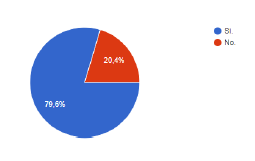
\includegraphics[width=8cm]{grafico}
		\end{center}
		\caption{Porcentaje de personas que aceptan la aplicaci�n m�vil}
		\label{grafico}
	\end{figure}
	
\end{enumerate}

%\subsection{Diagrama de Pantallas}
\chapter{Marco Te�rico}
En este cap�tulo se presentan los conceptos fundamentales para el desarrollo del sistema de riego automatizado.
\section{Sistema de riego}
Es el conjunto de estructuras, que permite determinar que �rea pueda ser cultivada aplic�ndole el agua necesaria a las plantas. Este consta de varios componentes. El conjunto de componentes depender� de si se trata de riego superficial, por aspersi�n, o por goteo.

\section{Ventajas de Instalar un Sistema de Riego}
\begin{itemize}
	\item Se logran altos grados de automatizaci�n, basados en el ahorro de mano de obra, agua y energ�a.
\item 	Los equipos son adaptables a cualquier tipo de terreno.
	\item Estos sistemas son adaptables a la rotaci�n de plantas y a riesgos estrat�gicos.
	\item Permite el crecimiento vertical de las plantas.
\end{itemize}

\section{Tipos de sistemas de riego}

\subsection{Riego por aspersi�n}

\begin{wrapfigure}[9]{l}{7cm}
	\begin{center}
		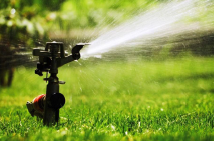
\includegraphics[width=6cm]{aspersion}
	
		\caption{Riego por aspersi�n}
\end{center}
	\label{as}
\end{wrapfigure}

Es aquel sistema de riego que trata de imitar a la lluvia. Es
decir, el agua destinada al riego se hace llegar a las plantas por medio de tuber�as y mediante unos pulverizadores, llamados aspersores y, gracias a una presi�n determinada, el agua se eleva para que luego caiga pulverizada o en forma de gotas sobre la superficie que se desea regar. En la Figura \ref{as} se puede apreciar un modelo de sistema de riego por aspersi�n.



\subsubsection{Ventajas de riego por aspersi�n}
\begin{itemize}
	\item Ahorro en mano de obra. Una vez puesto en marcha no necesita especial atenci�n. Existen en el mercado eficaces programadores activados por electrov�lvulas conectadas a un reloj que, por sectores y por tiempos, activar�a el sistema seg�n las necesidades previamente programadas, con lo cual la mano de obra es pr�cticamente
	inexistente.
	\item Adaptaci�n al terreno. Se puede aplicar tanto a terrenos lisos como a los ondulados, no necesitando allanamiento ni preparaci�n de las tierras.
	\item La eficiencia del riego por aspersi�n. Es de un 80\% frente al 50\% en los riegos por inundaci�n tradicionales. En consecuencia, el ahorro en agua es un factor muy importante a la hora de valorar este sistema.
	\item Especialmente �til para distintas clases de suelos. Ya que permite riegos frecuentes y poco abundantes en superficies poco permeables.
	\end{itemize}
	
\subsection{Riego por goteo autom�tico}
\begin{wrapfigure}[9]{r}{7cm}
	\begin{center}
		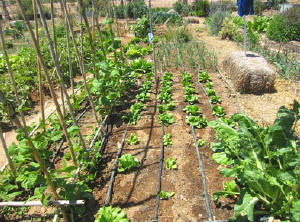
\includegraphics[width=6cm]{goteo}
	\end{center}
	\caption{Riego por goteo autom�tico}
	\label{goteo}
\end{wrapfigure}
	El riego por goteo (Figura \ref{goteo}) consiste en colocar tubos en hilera cerca de los tallos de las plantas y a trav�s de los goteros que se insertan en los tubos o tuber�as el agua va fluyendo gota a gota de una manera constante o por tiempo limitado, seg�n c�mo lo
programemos. Las tuber�as pueden estar enterradas ligeramente o colocadas de manera superficial sobre la tierra.


\subsubsection{Ventajas del riego por goteo autom�tico}
\begin{itemize}
	\item Se ahorra tiempo y esfuerzo en regar y puedes dedicarte a otras labores en el huerto o jard�n al tener la opci�n de automatizar los riegos.
	\item Se ahorra agua y se hace un uso m�s sostenible y eficiente de �sta al ser un m�todo de riego de bajo consumo.
	\item El riego por goteo permite llevar a cabo la fertirrigaci�n a la vez que se riega, es decir, aportar al agua preparados con nutrientes para mejorar la fertilidad de la tierra o para prevenir y combatir plagas y enfermedades.
	\item Las ra�ces de las plantas con riego por goteo tienden a crecer de manera vertical o	profunda en lugar de horizontal o paralela al suelo, llegando a acceder a los nutrientes de las capas m�s profundas del suelo y a almacenar m�s agua.
	\item	Como no se mojan las partes �ereas de las plantas, no hay problemas de que �stas	se quemen por el sol una vez mojadas o que aparezcan plagas y enfermedades.
		\item Como podemos programar y automatizar los riegos, este sistema es ideal para cuando no podemos atender el huerto o jard�n o nos vamos de vacaciones y que nuestras plantas sigan recibiendo agua.
\item 	Un sistema de riego por goteo se puede usar y adaptar a todo tipo de huertos y jardines.
\end{itemize}
\section{Riego de superficie}
El riego por superficie (o de gravedad) contin�a teniendo una importancia relevante en el desarrollo del regad�o, no s�lo porque corresponde aproximadamente al 80\% de las �reas regadas del Mundo, sino porque contin�a siendo el m�todo m�s apropiado, t�cnicamente, para suelos llanos y pesados, y, econ�micamente, para muchos cultivos y sistemasde producci�n. Los sistemas de riego de gravedad son muchos, en correspondencia con los procesos de aplicaci�n del agua a las parcelas regadas. Estos se resumen esencialmente a los sistemas de surcos, canteros, fajas, surcos a nivel y riego de esparcimiento. Los sistemas de surcos y fajas son llamados de infiltraci�n porque se aplican caudales suficientemente grandes, para que el agua fluya sobre el terreno, y, sucientemente peque�os, para que se vaya infiltrando mientras fluye, de forma que el agua deja de estar sobre el terreno en cuanto se corta el suministro. Se trata, pues, de riego de larga duraci�n, al contrario del riego por canteros.

\subsection{Factores que influyen en el sistema de riego}
\begin{itemize}
	\item Profundidad de las ra�ces: El volumen de agua almacenado por cada tipo de suelo se va a ser aprovechado de distinta manera en funci�n de la planta, de su superficie foliar y del desarrollo y la profundidad efectiva de su sistema radicular, principalmente.
	Es por este motivo por el que debemos considerar estos aspectos para determinar	los vol�menes de agua precisos a aportar en los distintos riegos y la frecuencia de los mismos. En la mayor�a de las plantas la profundidad efectiva de las ra�ces se encuentra entre los 50 y 100 cm.
	\item Textura del suelo: indica el contenido relativo de part�culas de diferente tama�o, como la arena, el limo y la arcilla, en el suelo. La textura tiene que ver con la facilidad con que se puede trabajar el suelo, la cantidad de agua y aire que retiene y la velocidad con que el agua penetra en el suelo y lo atraviesa.
\item 	Temperatura media: La velocidad del crecimiento de las plantas la determina la	temperatura diurna promedio. Para determinar este promedio se debe multiplicar la temperatura diurna promedio por el n�mero de horas de luz del d� am�s la temperatura nocturna promedio multiplicada por el n�mero de horas de oscuridad divido por 24.
\item 	Humedad relativa: Los niveles de humedad uct�an con el cambio de la temperatura del aire y, adem�s, las plantas transpiran y agregan vapor de agua al ambiente constantemente. En las �reas clim�ticas del norte, estos desaf�os se multiplican por muchos factores, como que el aire exterior m�s seco es demasiado fr�o para realizar intercambios de aire. El aire h�medo contribuye directamente a los problemas, como
enfermedades de las ra�ces y las hojas, secado lento del sustrato, estr�s de las plantas, p�rdida de calidad, p�rdida de producci�n, etc. Por lo tanto, se necesitan m�s pesticidas para el control de las enfermedades y las plantas tender�n a tener un crecimiento d�bil y estirado, lo que las har�a menos atractivas. Si la humedad es demasiado baja, con frecuencia el crecimiento de las plantas se ver�a afectado.
Adem�s, a menudo se caen las hojas inferiores, el crecimiento es dif�cil y la calidad en general no es muy buena.
\end{itemize}

\subsection{Raspberry}
\begin{wrapfigure}[8]{l}{7cm}
	\begin{center}
		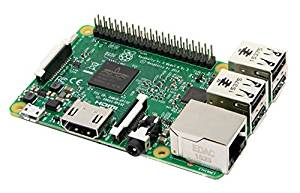
\includegraphics[width=6cm]{ras}
	\end{center}
	\caption{Raspberry Pi 3}
	\label{ras}
\end{wrapfigure}
Raspberry PI es una placa computadora (SBC) de bajo coste, se podr�a decir que es un ordenador de tama�o reducido, del orden de una tarjeta de cr�dito, desarrollado en el Reino Unido por la Fundaci�n Raspberry PI (Universidad de Cambridge) en 2011, con el objetivo de estimular la ense�anza de la inform�tica en las escuelas, aunque no empez� su comercializaci�n hasta el a�o 2012.
El concepto es el de un ordenador desnudo de todos los accesorios que se pueden eliminar sin que afecte al funcionamiento b�sico. Est� formada por una placa que soporta varios componentes necesarios en un ordenador com�n y es capaz de comportarse como tal.
Una Raspberry es tambi�n un sistema digital de procesamiento y que funciona gracias a un sistema operativo. 
En esencia, el Raspberry Pi es una placa de un tama�o min�sculo, posee un micro procesador ARM con potencia de hasta 1GHz, integrado en un chip Broadcom BCM2835. Adem�s cuenta con 512 MB de RAM, un GPU Videocore IV, todo lo necesario para poder ejecutar programas b�sicos, navegar por internet y por supuesto programar.
Para trabajar con un Raspberry Pi se requiere almacenamiento que en este caso espec�fico debe ser una tarjeta de memoria SD o microSD. Al contar con todos estos elementos, s�lo debe conectarse a la corriente el�ctrica. Las placas m�s modernas cuentan con hasta 4 puertos USB para conectar teclado y mouse, un conector HDMI con capacidad de  reproducir v�deo en 1080p y hasta una conexi�n Ethernet para poder tener internet v�a cable.

\subsubsection{Ventajas de la Raspberry}
\begin{itemize}
	\item Bajo consumo, aproximadamente consume 700mA (sin accesorios ni overclocking), lo que nos permite tenerlo encendido.
	\item Bajo precio,  es accesible para todos y es m�s rentable comprar uno para propios proyectos que pagar un servidor por ejemplo.
	\item Accesorios de f�cil disponibilidad. Siendo su fuente de alimentaci�n un cargador de un m�vil y su almacenamiento una memoria SD, podemos decir que cualquiera tiene esto en casa.
	\item Tama�o reducido. La placa completa puede ser algo m�s grande que una tarjeta de cr�dito, lo que permite llevarla a cualquier sitio e instalarla en lugares con poco espacio.
	\item Cuenta con la mayor�a de programas que podemos tener en linux, como apache, samba, mysql, transmission,xbmc etc.
\end{itemize}

\section{Sensor de temperatura DS18B20}
El sensor de temperatura DS18B20 es un dispositivo que se comunica de forma digital. Cuenta con tres terminales, los dos de alimentaci�n y el pin data. Con Arduino se lee la temperatura que registra este sensor que posee la caracter�stica onewire.

\begin{wrapfigure}[10]{r}{7cm}
	\begin{center}
		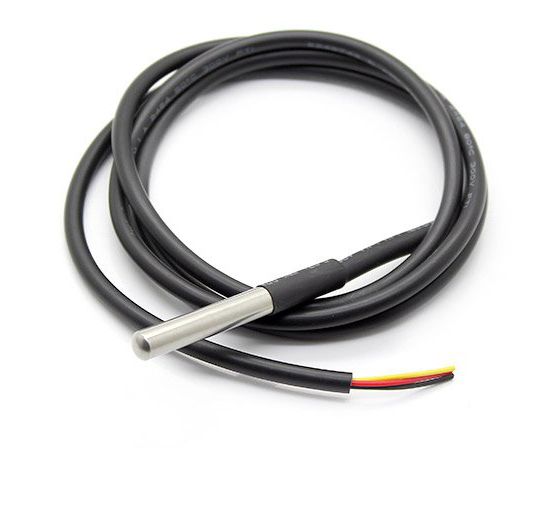
\includegraphics[width=6cm]{sensor1}
	\end{center}
	\caption{Sensor de temperatura DS18B20}
	\label{s1}
\end{wrapfigure}  

\subsubsection{Caracter�sticas}
\begin{itemize}
\item 	Es un term�metro digital de alta precisi�n, entre 9 y 12 bits de temperatura en grados Celsius (el usuario puede escoger la precisi�n deseada).
	\item Su temperatura operativa se encuentra entre 50 y 125 grados Celsius. La precisi�n, en el rango comprendido entre 10 y 85 grados es de 0.5 grados.
\item 	Se puede escoger entre el modelo sumergible y los modelos para uso en placas de circuitos.
\end{itemize}

\section{Sensor de humedad FC28}
\begin{wrapfigure}[10]{l}{6cm}
	\begin{center}
		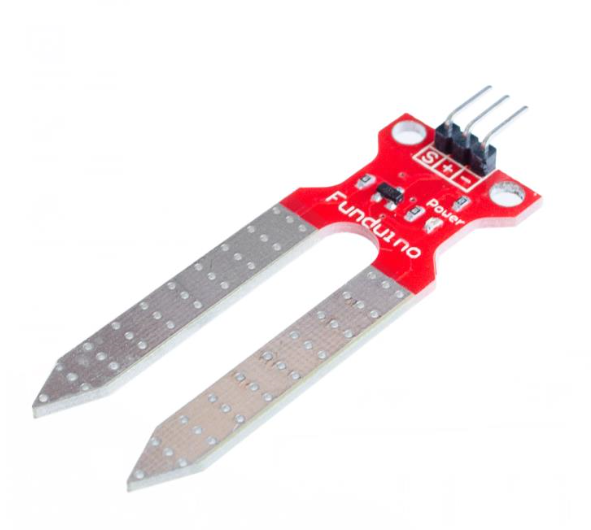
\includegraphics[width=5cm]{sensor2}
	\end{center}
	\caption{Sensor de humedad FC28}
	\label{s2}
\end{wrapfigure}
Con este sensor se implementa un sistema para hacer que indique cuando este demasiado seca la tierra y as� automatizar el proceso de regado
de las plantas, o tambi�n se adecua a la necesidad puntual que tengas ya que es completamente compatible con Arduino u otro controlador.
Este sensor utiliza las dos sondas para pasar corriente a trav�s del suelo, y luego se lee que la resistencia para obtener el nivel de humedad. M�s agua hace que la electricidad pase m�s f�cilmente
(menos resistencia), mientras que el suelo seco conduce mal la electricidad (mayor resistencia).
  
\subsubsection{Caracter�sticas}
\begin{itemize}
\item Voltaje de funcionamiento: 3.3v - 5v
\item Se�al de salida: 0 - 4.2 v
\item Consumo de corriente: 35mA
\end{itemize}

\section{Sensor de flujo YF-S201}

El YF-S201 es un sensor de flujo de construcci�n s�lida el cual esta constituido por un cuerpo de pl�stico, un rotor de agua, y un sensor de efecto Hall.\\
\begin{wrapfigure}[8]{r}{7cm}
	\begin{center}
		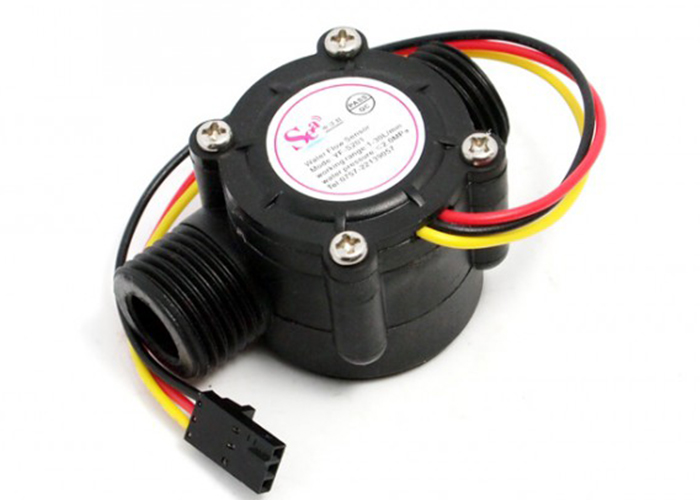
\includegraphics[width=6cm]{sensor3.jpg}
	\end{center}
	\caption{Sensor de flujo YF-S201}
	\label{s3}
\end{wrapfigure}  
El dise�o y el funcionamiento de este tipo de sensor es simple. Utiliza un sensor con aspas o �labes para medir la cantidad de l�quido que se ha movido a trav�s de �l. El molino de viento tiene un peque�o im�n atado y hay un sensor magn�tico de efecto Hall en el otro lado del tubo que registra cada vuelta del molino de viento, esto genera impulsos de
salida a una velocidad proporcional a la velocidad de flujo.
Al contar los pulsos de la salida del sensor, puede seguir f�cilmente el movimiento del ruido: cada pulso es de aproximadamente 2,25 mililitros.
El YF-S201 es adecuado para un tubo est�ndar de 1/2 y se puede insertar f�cilmente en un sistema de tuber�as est�ndar.

\section{Modulo RTC DS3231}
\begin{wrapfigure}[9]{l}{6cm}
	\begin{center}
		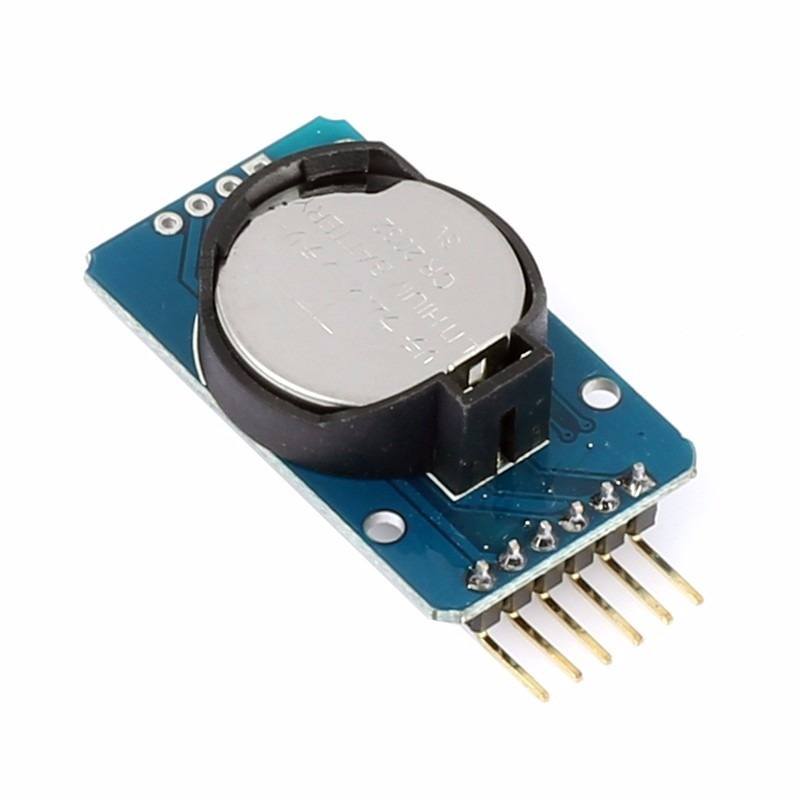
\includegraphics[width=5cm]{sensor4.jpg}
	\end{center}
	\caption{Modulo RTC DS3231}
	\label{s4}
\end{wrapfigure}  
Es un reloj en tiempo real (RTC) de bajo costo y gran
precisi�n con oscilador de cristal compensado por temperatura (TCXO) y cristal integrado. El dispositivo incorpora una entrada de bater�a y mantiene un reloj preciso cuando se interrumpe la alimentaci�n principal del dispositivo.
La integraci�n del resonador de cristal mejora la precisi�n a largo plazo del dispositivo.
El RTC mantiene la informaci�n de los segundos, minutos, horas, d�a, fecha, mes y a�o. La fecha al final del mes se ajusta autom�ticamente para los meses con menos de 31 d�as, incluyendo las correcciones para el a�o bisiesto. El reloj funciona en formato de 24 horas o 12 horas con un indicador AM/PM. Se proporcionan dos alarmas programables de hora del d�a y una salida de onda cuadrada programable. La direcci�n y los datos se transfieren en serie a trav�s de un bus bidireccional I2C.
Una referencia de voltaje compensada por temperatura de precisi�n y un circuito comparador monitorean el estado del VCC para detectar fallas de energ�a, proporcionar una salida de reajuste y cambiar autom�ticamente a la fuente de reserva cuando sea necesario.


\section{Fotoresistencia}
\begin{wrapfigure}[7]{l}{6cm}
	\begin{center}
		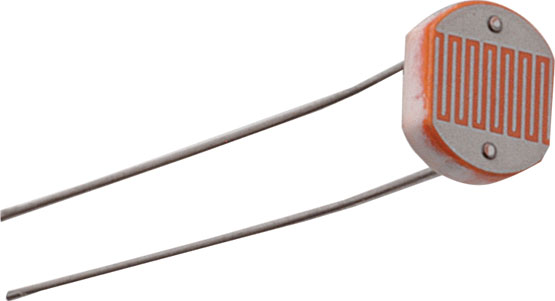
\includegraphics[width=5cm]{sensor5.jpg}
	\end{center}
	\caption{Fotoresistencia}
	\label{s5}
\end{wrapfigure}
El LDR (Light Dependent Resistor) o fotoresistencia es una resistencia que var�a su resistencia en funci�n de la luz que incide sobre su superficie. Cuanto mayor sea la intensidad de la luz que incide en la superficie del LDR menor ser� su resistencia y cuanto menos luz incida mayor ser� su resistencia.
Cuando la LDR no est� expuesta a radiaciones luminosas los electrones est�n firmemente unidos en los �tomos que la conforman pero cuando sobre ella inciden radiaciones luminosas esta energ�a libera electrones con lo cual el material se hace m�s conductor, y de esta manera disminuye su resistencia. Las resistencias LDR solamente reducen su resistencia con una radiaci�n luminosa situada dentro de una determinada banda de longitudes de onda. Las construidas con sulfuro de cadmio son sensibles a todas las radiaciones luminosas visibles, las construidas con sulfuro de plomo solamente son sensibles a las radiaciones infrarrojas.



\section{M�dulo Sensor de Nivel de Agua}
\begin{wrapfigure}[11]{r}{6cm}
	\begin{center}
		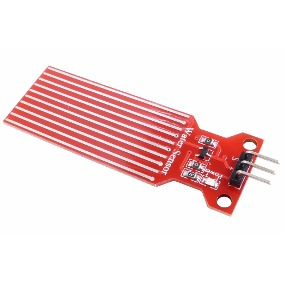
\includegraphics[width=5cm]{sensor6.jpg}
	\end{center}
	\caption{M�dulo Sensor de Nivel de Agua}
	\label{s6}
\end{wrapfigure}
El sensor de agua est� dise�ado para la detecci�n de agua y se puede usar para confirmar la presencia de lluvia, nivel de agua en un determinado punto o alerta por fuga de agua.
B�sicamente el sensor de agua se compone de un conector, un bloque resitivo de 1 Mega Ohms y una serie de l�neas conductivas.
Las lineas conductivas si detectan agua cierran el circuito interno dando una ca�da de tensi�n que podemos leer por el pin de se�al.

En otras palabras, el sensor de agua sirve para leer un nivel de agua variando a lo largo de sus l�minas conductoras de manera que conectado a una entrada anal�gica nos devolver� diferentes valores de tensi�n dependiendo de la cantidad de agua que cubra la zona de l�minas paralelas.

\subsection{Caracter�sticas}
\begin{itemize}
	\item Alimentaci�n: 3 - 5V
\item	Consumo: menor que 20mA
\item 	Deteci�n anal�gica
\item 	Area de detecci�n 40 x 16mm
\item	Temperatura de trabajo: 10 - 30�C
\end{itemize}

\chapter{Pruebas y Resultados}
En este cap\'itulo se describen las pruebas realizadas al prototipo del sistema de riego para verificar su funcionamiento, as\'i como se comenta los resultados obtenidos de las mismas. 

\section{Pruebas}

\subsection{Control individual de los sensores del sistema de riego con Raspberry}
Inicialmente, para comprobar el funcionamiento de los sensores en Raspberry, cada uno de ellos se prob\'o individualmente en la tarjeta. Para realizar lo anterior, a cada sensor se le asignaron unos pines de uso, de forma que en un futuro pudieran integrarse todos juntos sin problema, y se les dise\~{n}o un peque\~{n}o script sin interfaz gr\'afica que se encargara de obtener y mostrar los datos del mismo.\\\\
En la figura \ref{r1}, se puede observar el proceso de desaroll\'o de uno de los scripts, todo esto dentro de la misma Raspberry.
\begin{figure}[H]
\begin{center}
	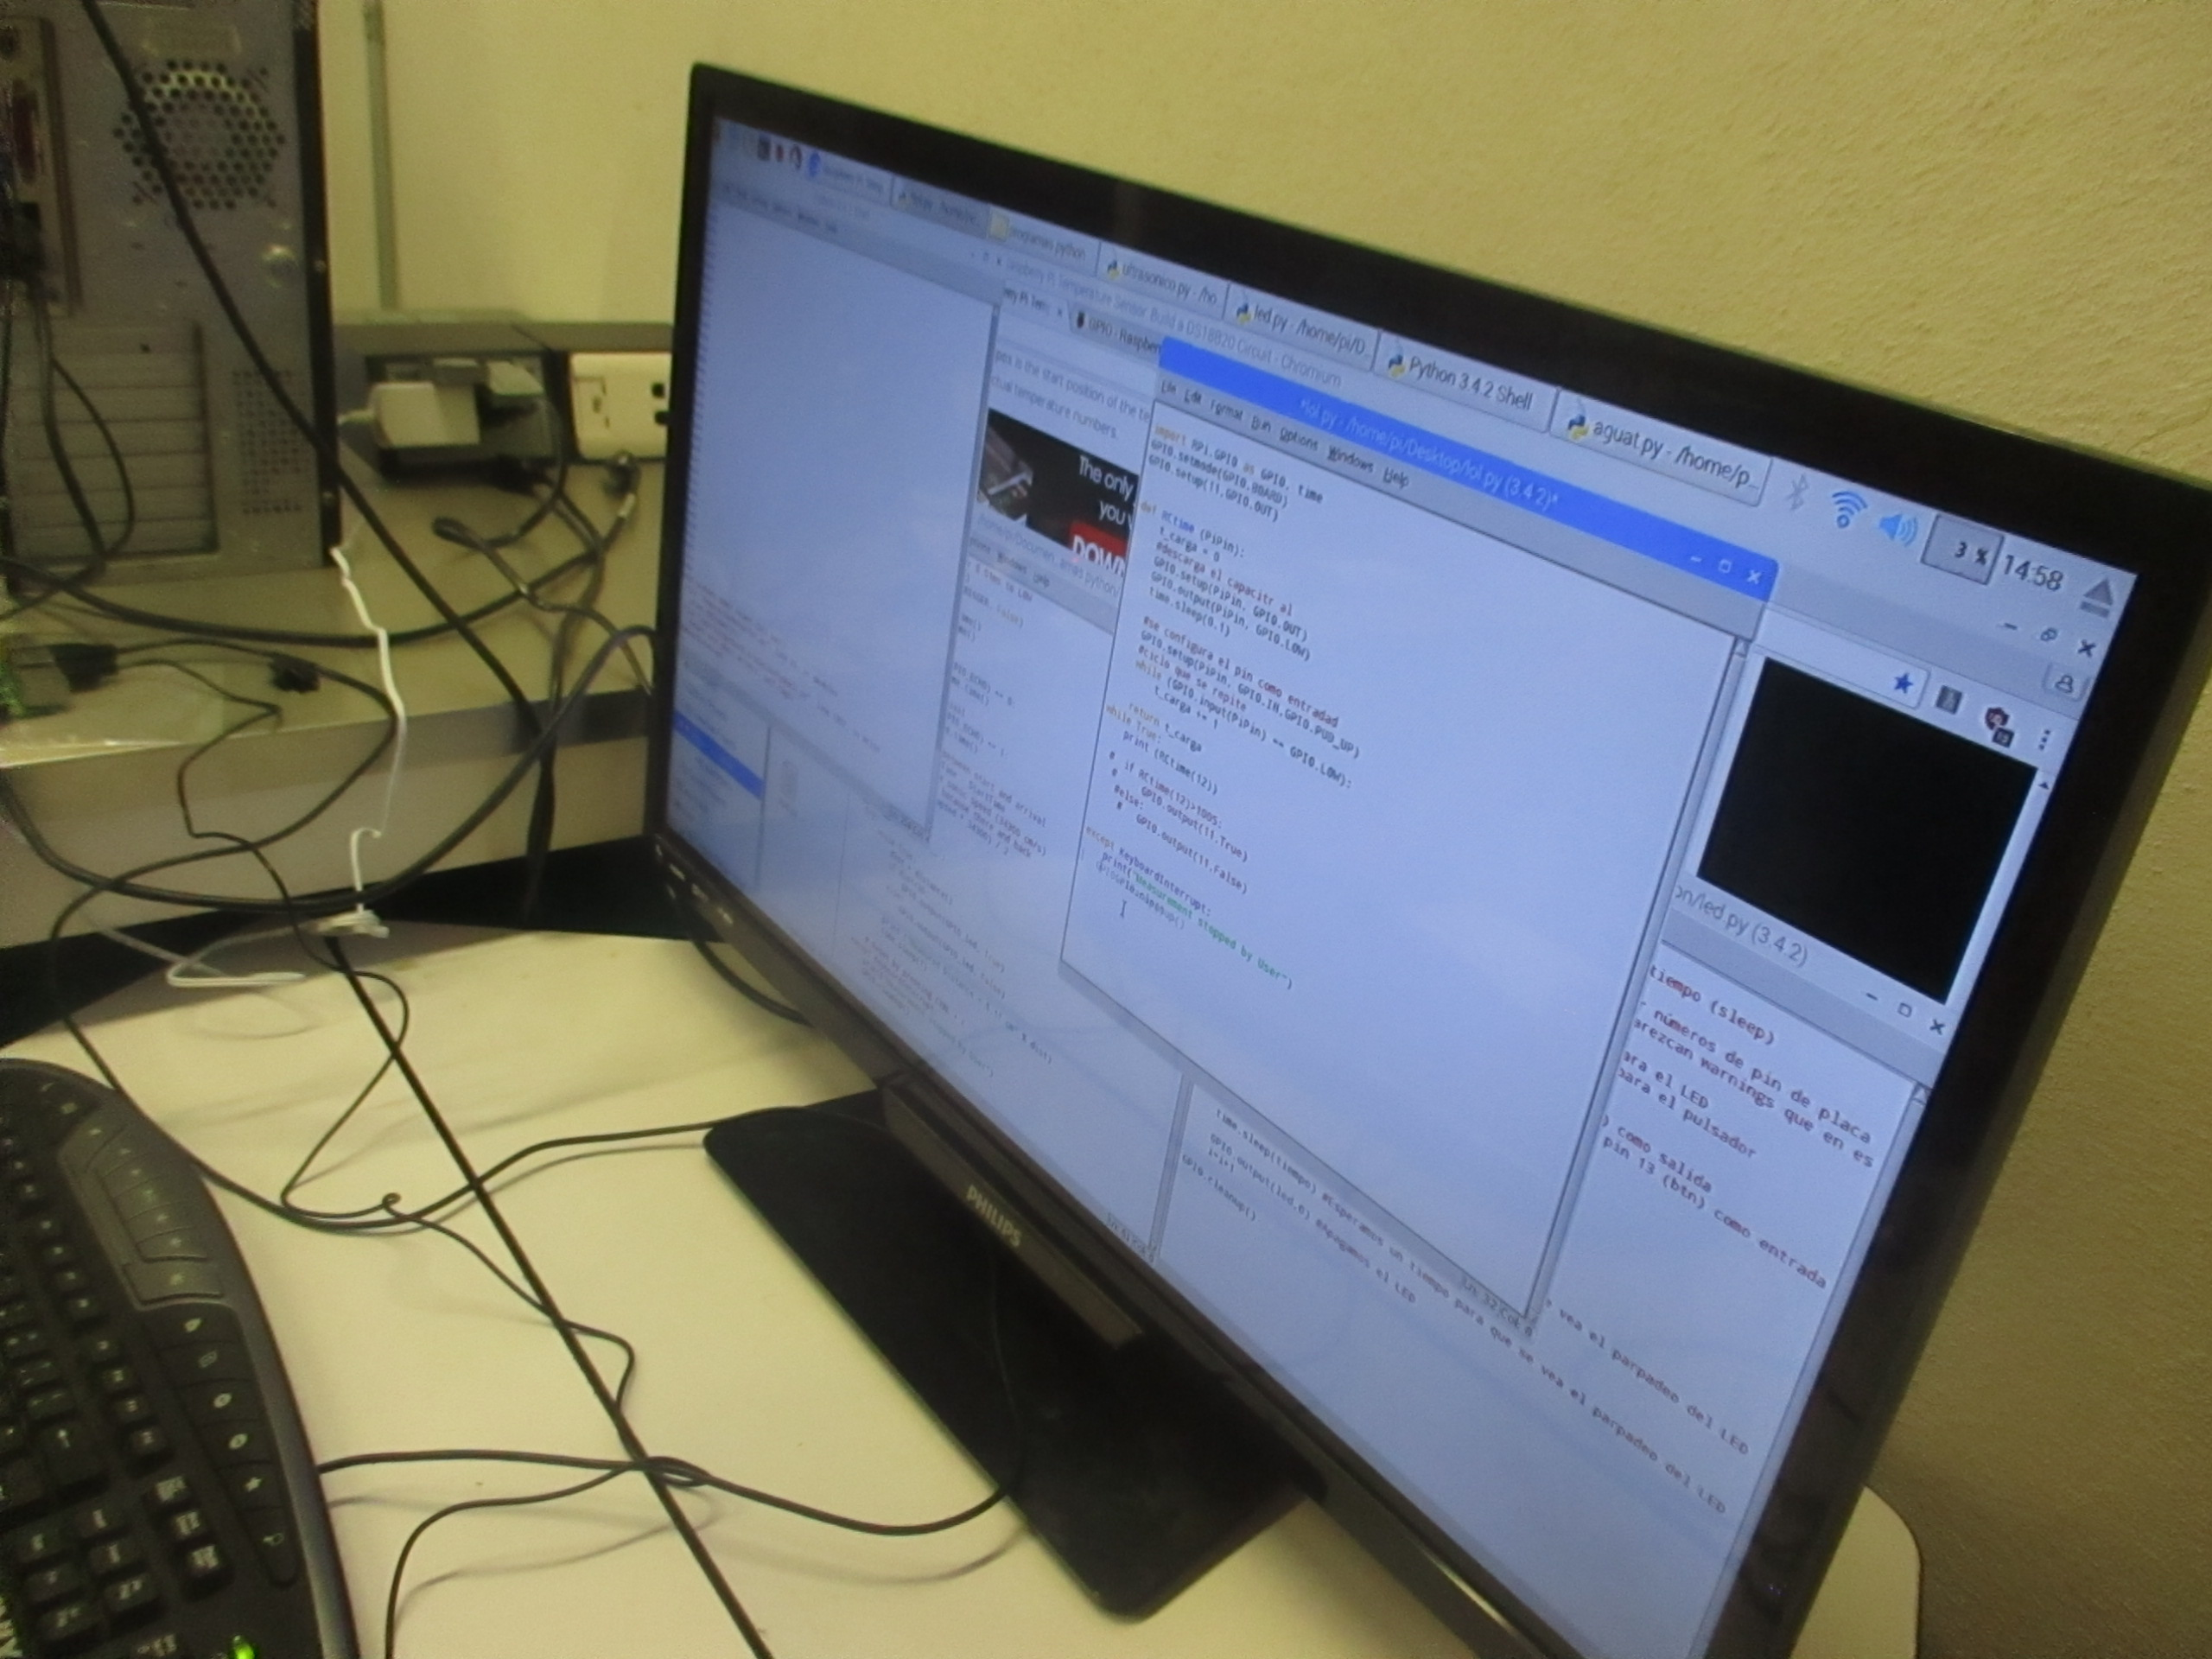
\includegraphics[width=7cm]{r1}
\end{center}
	\caption{Desarrollo del script para el sensor de flujo de agua.}
	\label{r1}
\end{figure} 
El resultado de ejecutar el script anterior, es mostrado en la figura \ref{r4}. El programa corresponde al sensor de flujo de agua y se encarga de mostrar la velocidad del paso de agua de litros por minuto.
\begin{figure}[H]
	\begin{center}
		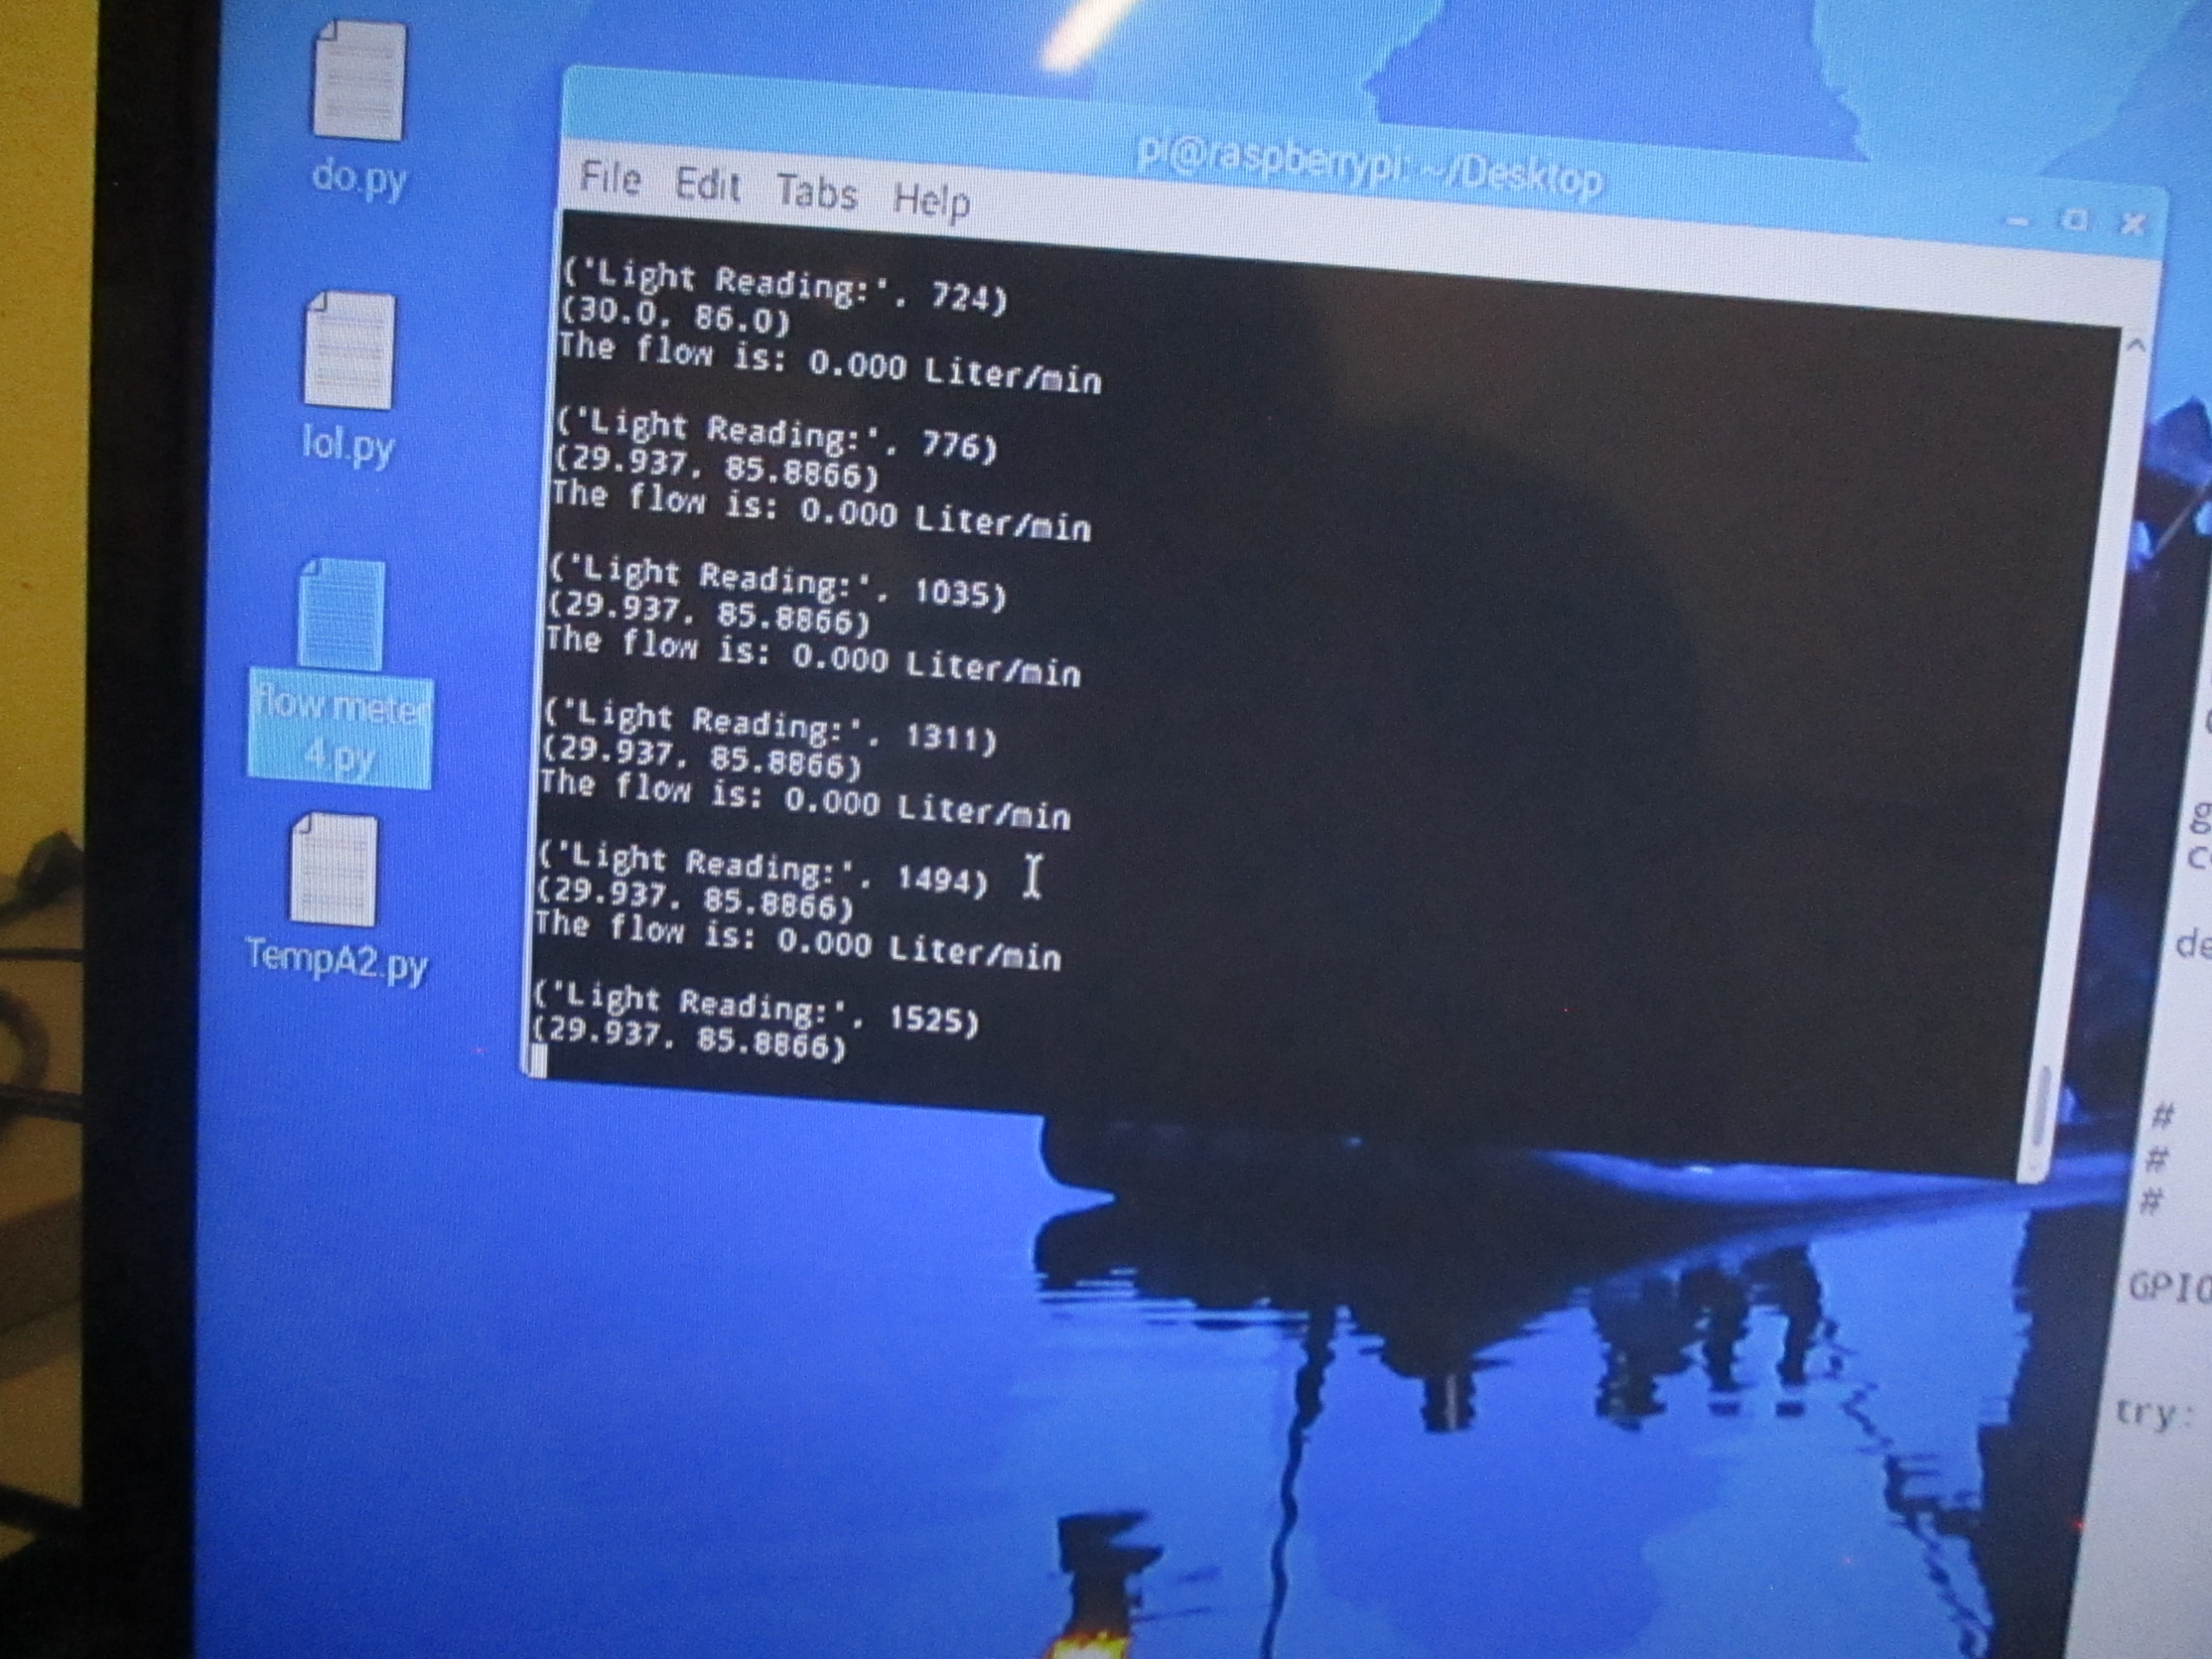
\includegraphics[width=7cm]{r4}
	\end{center}
	\caption{Prueba de funcionamiento del script del sensor de flujo de agua.}
	\label{r4}
\end{figure} 

\subsection{Control grupal de los sensores del sistema de riego con Raspberry}
En la siguiente etapa de desarroll\'o, todos los sensores fueron integrados a la Raspberry. Con base en lo anterior, se realizaron peque\~{n}as pruebas en las que, de uno en uno, cada sensor se acoplaba en su espacio correspondiente en la tarjeta y su c\'odigo de funcionamiento era a\~{n}adido a un script maestro.\\ 
El dise\~{n}o inicial de la Raspberry con todos los sensores integrados puede ser observado en la imagen \ref{todo} (a), mientras que la primera versi\'on del script maestro se puede visualizar en la imagen \ref{todo} (b). 
 
\begin{figure}[H]
	\begin{center}
		\subfigure[Sensores conectados a la Raspberry.]{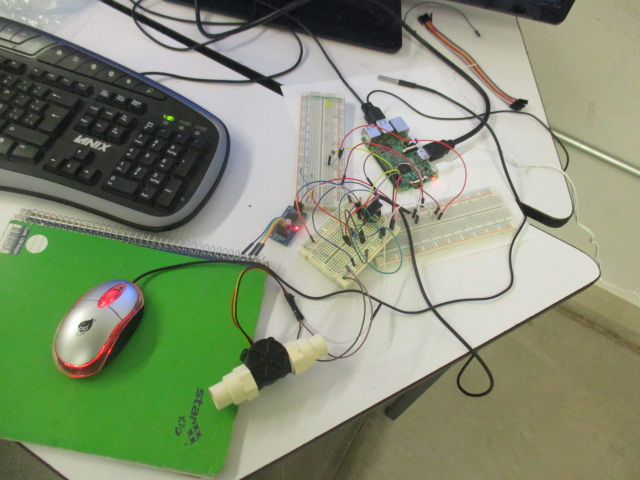
\includegraphics[width=7.5cm]{proto2}}
		\subfigure[Funcionamiento del script maestro.]{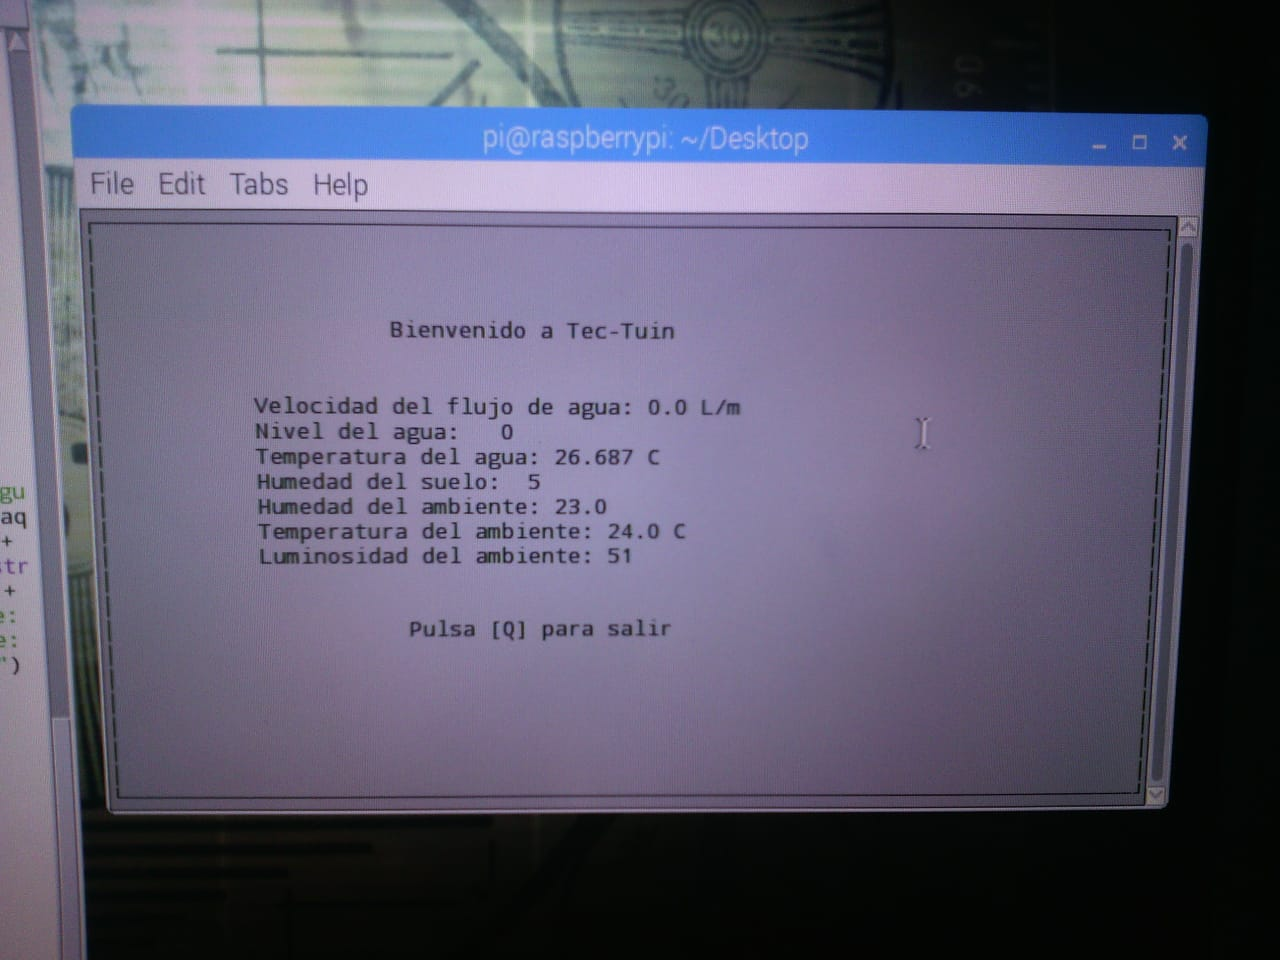
\includegraphics[width=7.5cm]{proto1}}
	\end{center}
	\label{todo}
	\caption{Primera versi\'on del prototipo de sistema de riego}
\end{figure} 


\subsection{Interpretaci\'{o}n de los datos obtenidos de los sensores del sistema de riego con Raspberry}
En las \'ultimas fases de desarrollo, con la Raspberry censando de manera correcta las variables del entorno, se empez\'o a desarrollar un c\'odigo para la interpretaci\'on de los datos obtenidos. Por ejemplo: si la humedad en el suelo es muy baja el riego comienza, en caso contrario el riego se detiene; si el nivel de agua disponible es muy bajo, el prototipo no acciona la bomba y manda un mensaje al usuario inform\'andole de lo acontecido. Para probar que lo anterior dicho sucede, se recrearon las condiciones necesarias para que cada uno de estos eventos suceda.

\begin{comment} 
Se puede observar en la imagen \ref{evento1} que, cuando el sensor de humedad del suelo reporta valores altos, el riego se detiene en el momento. 

\begin{figure}[H]
	\begin{center}
		\subfigure[Detecci\'on de un nivel alto de humedad del suelo.]{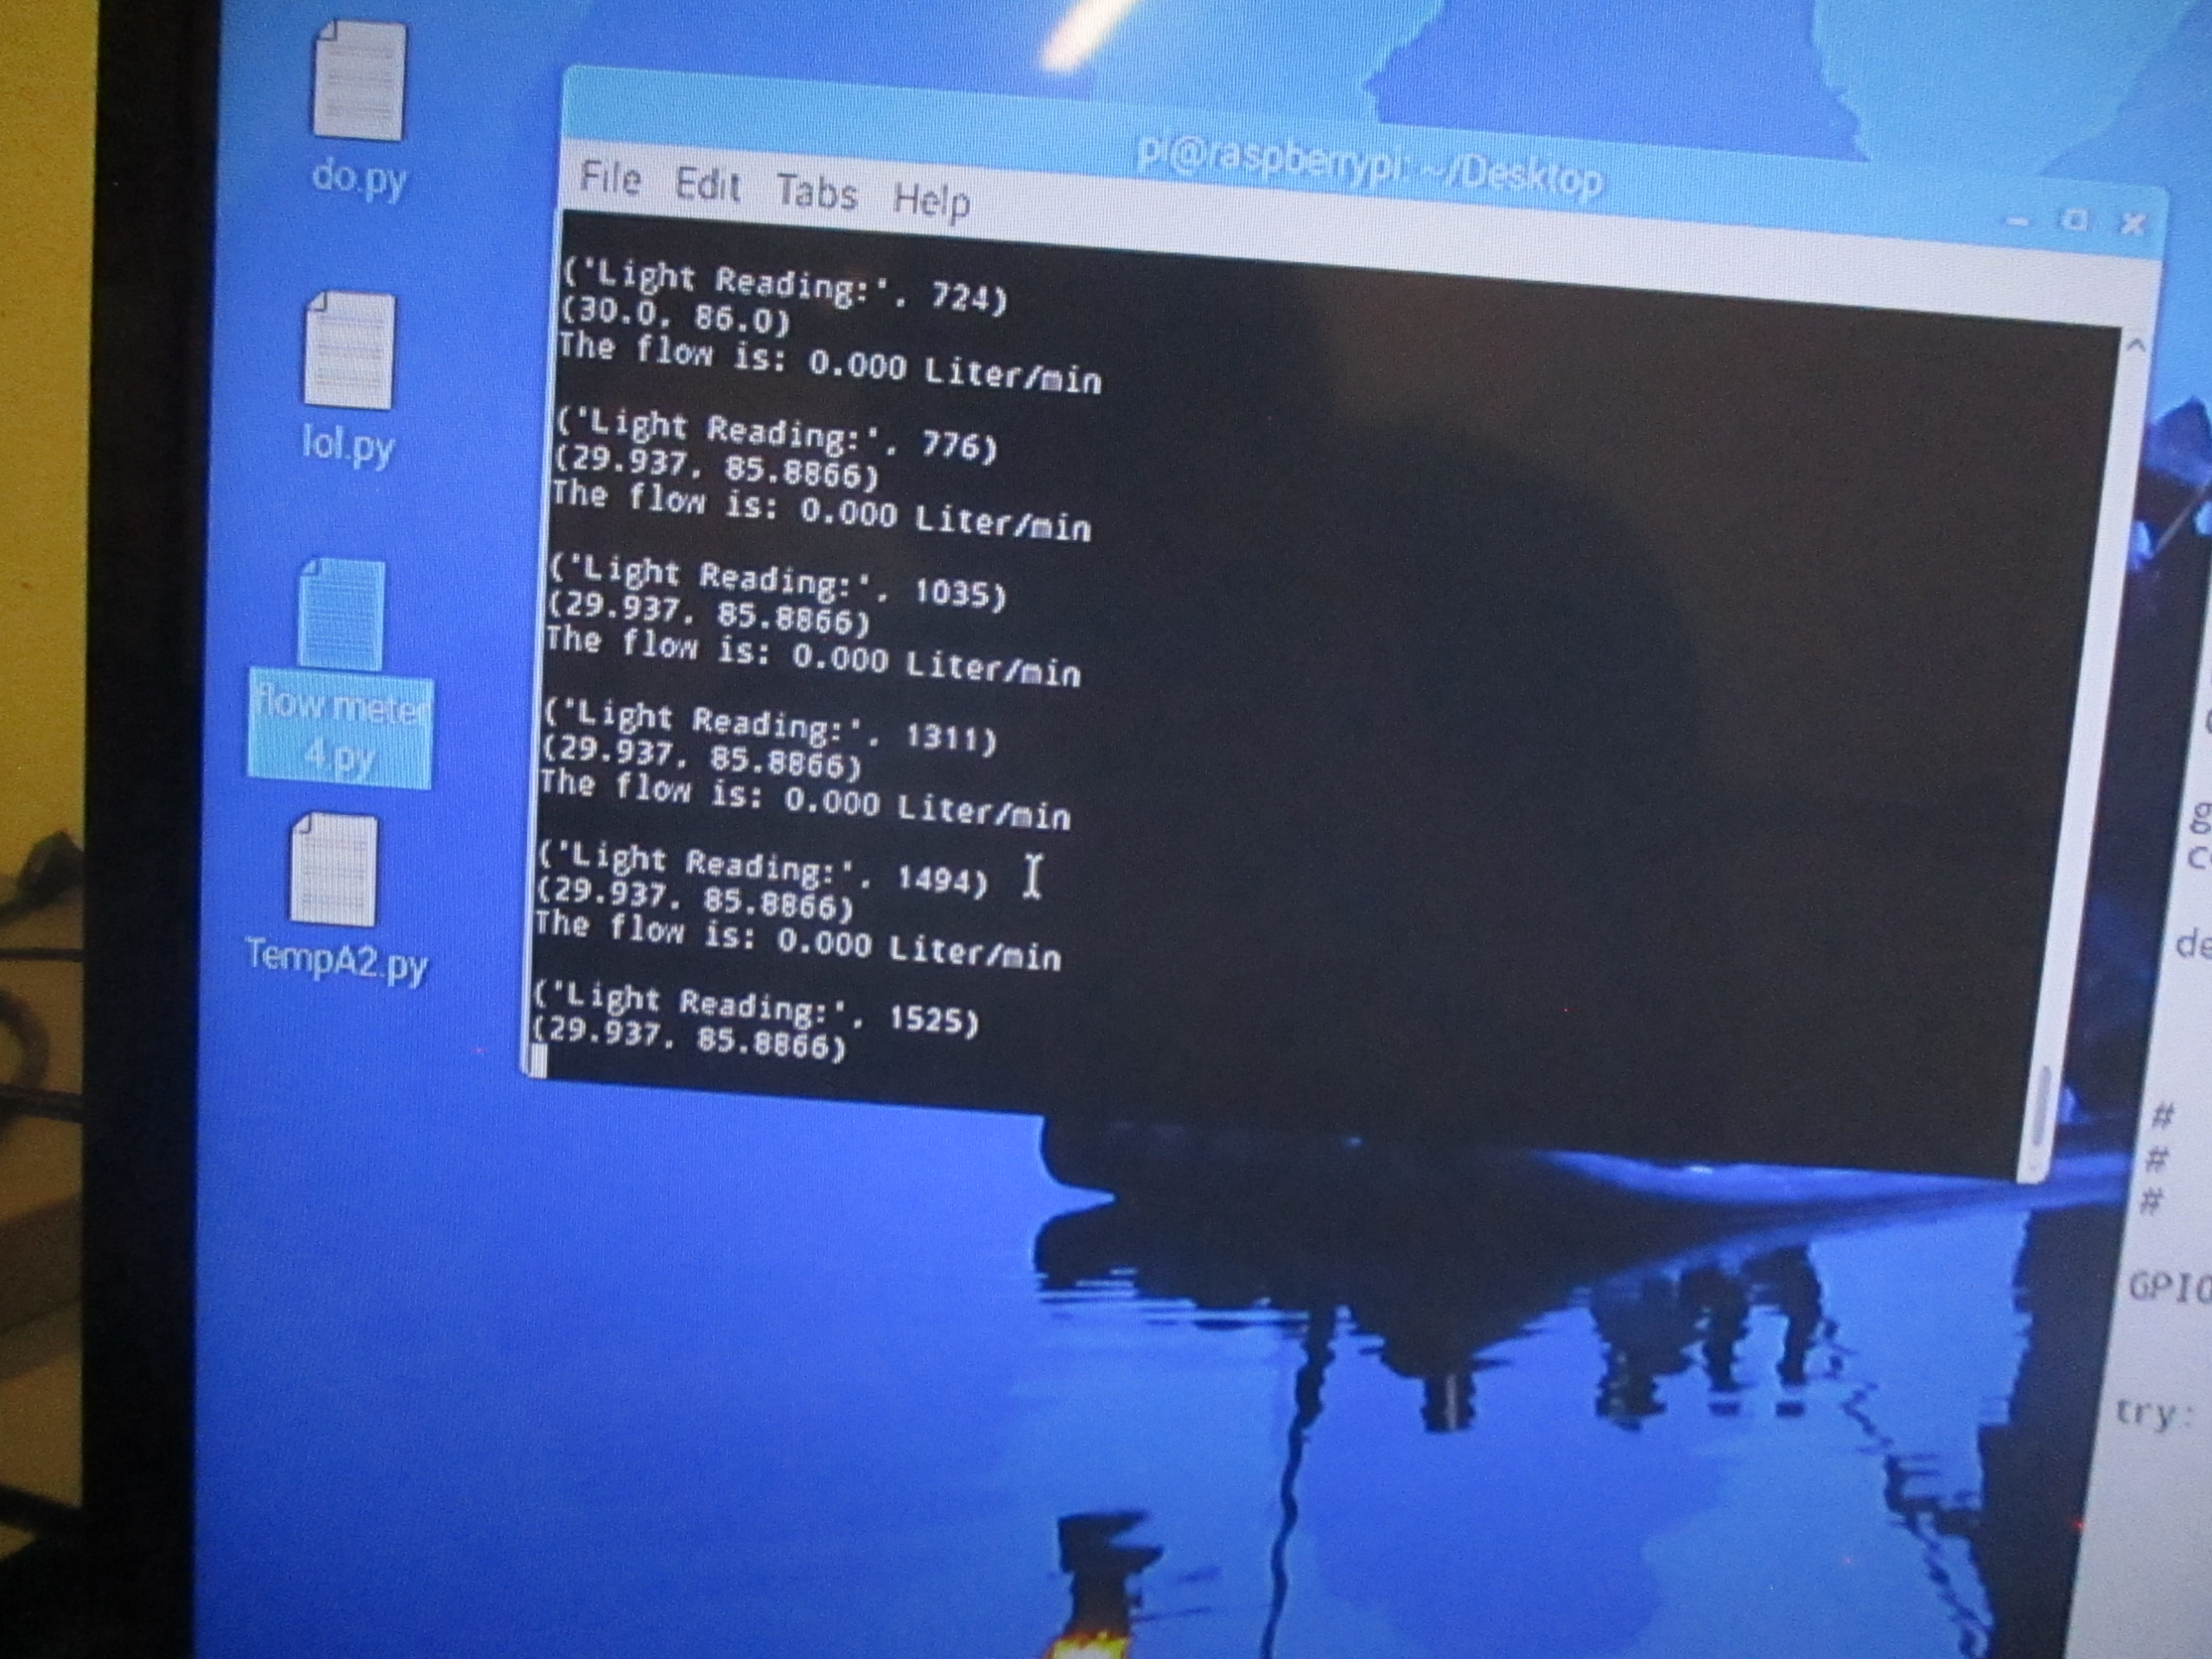
\includegraphics[width=7.5cm]{r4}}
		\subfigure[Riego detenido.]{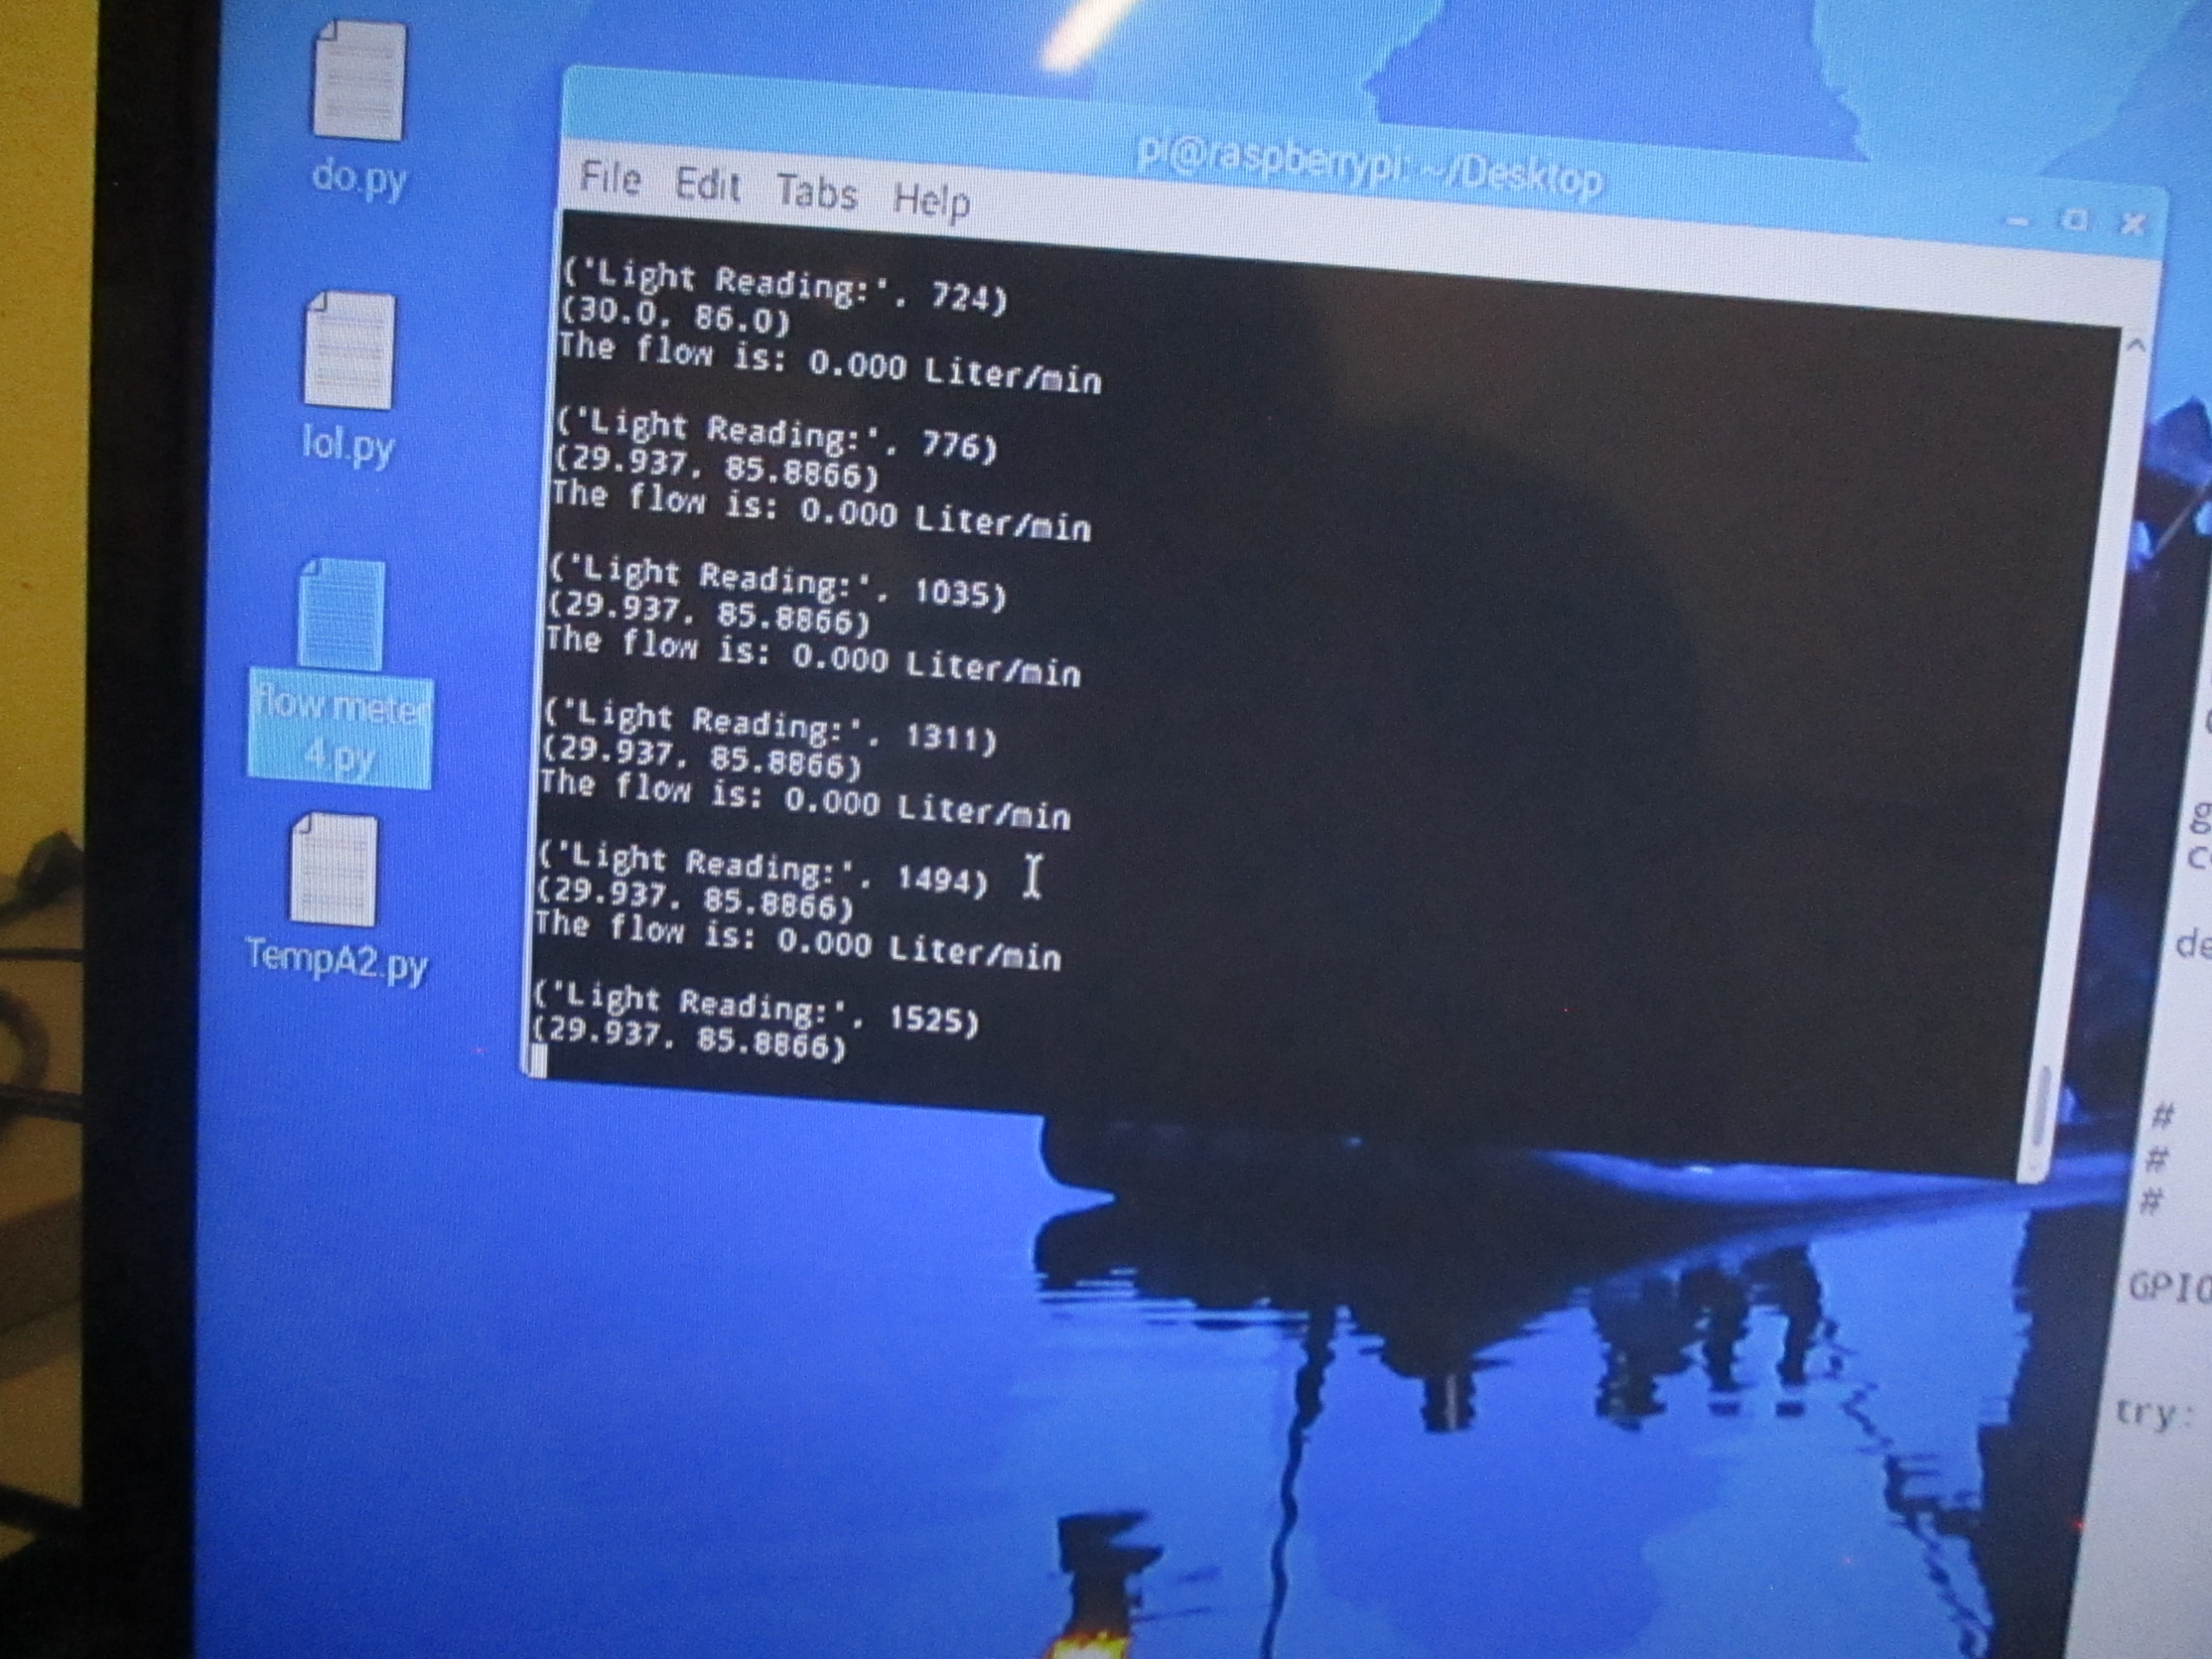
\includegraphics[width=7.5cm]{r4}}
	\end{center}
	\label{evento1}
	\caption{Primera evento considerado.}
\end{figure} 

En caso de que se detecten valores bajos de humedad en el suelo como en la imagen \ref{evento2}, el riego dar\'a inicio de manera autom\'atica. 

\begin{figure}[H]
	\begin{center}
		\subfigure[Detecci\'on de un nivel bajo de humedad del suelo.]{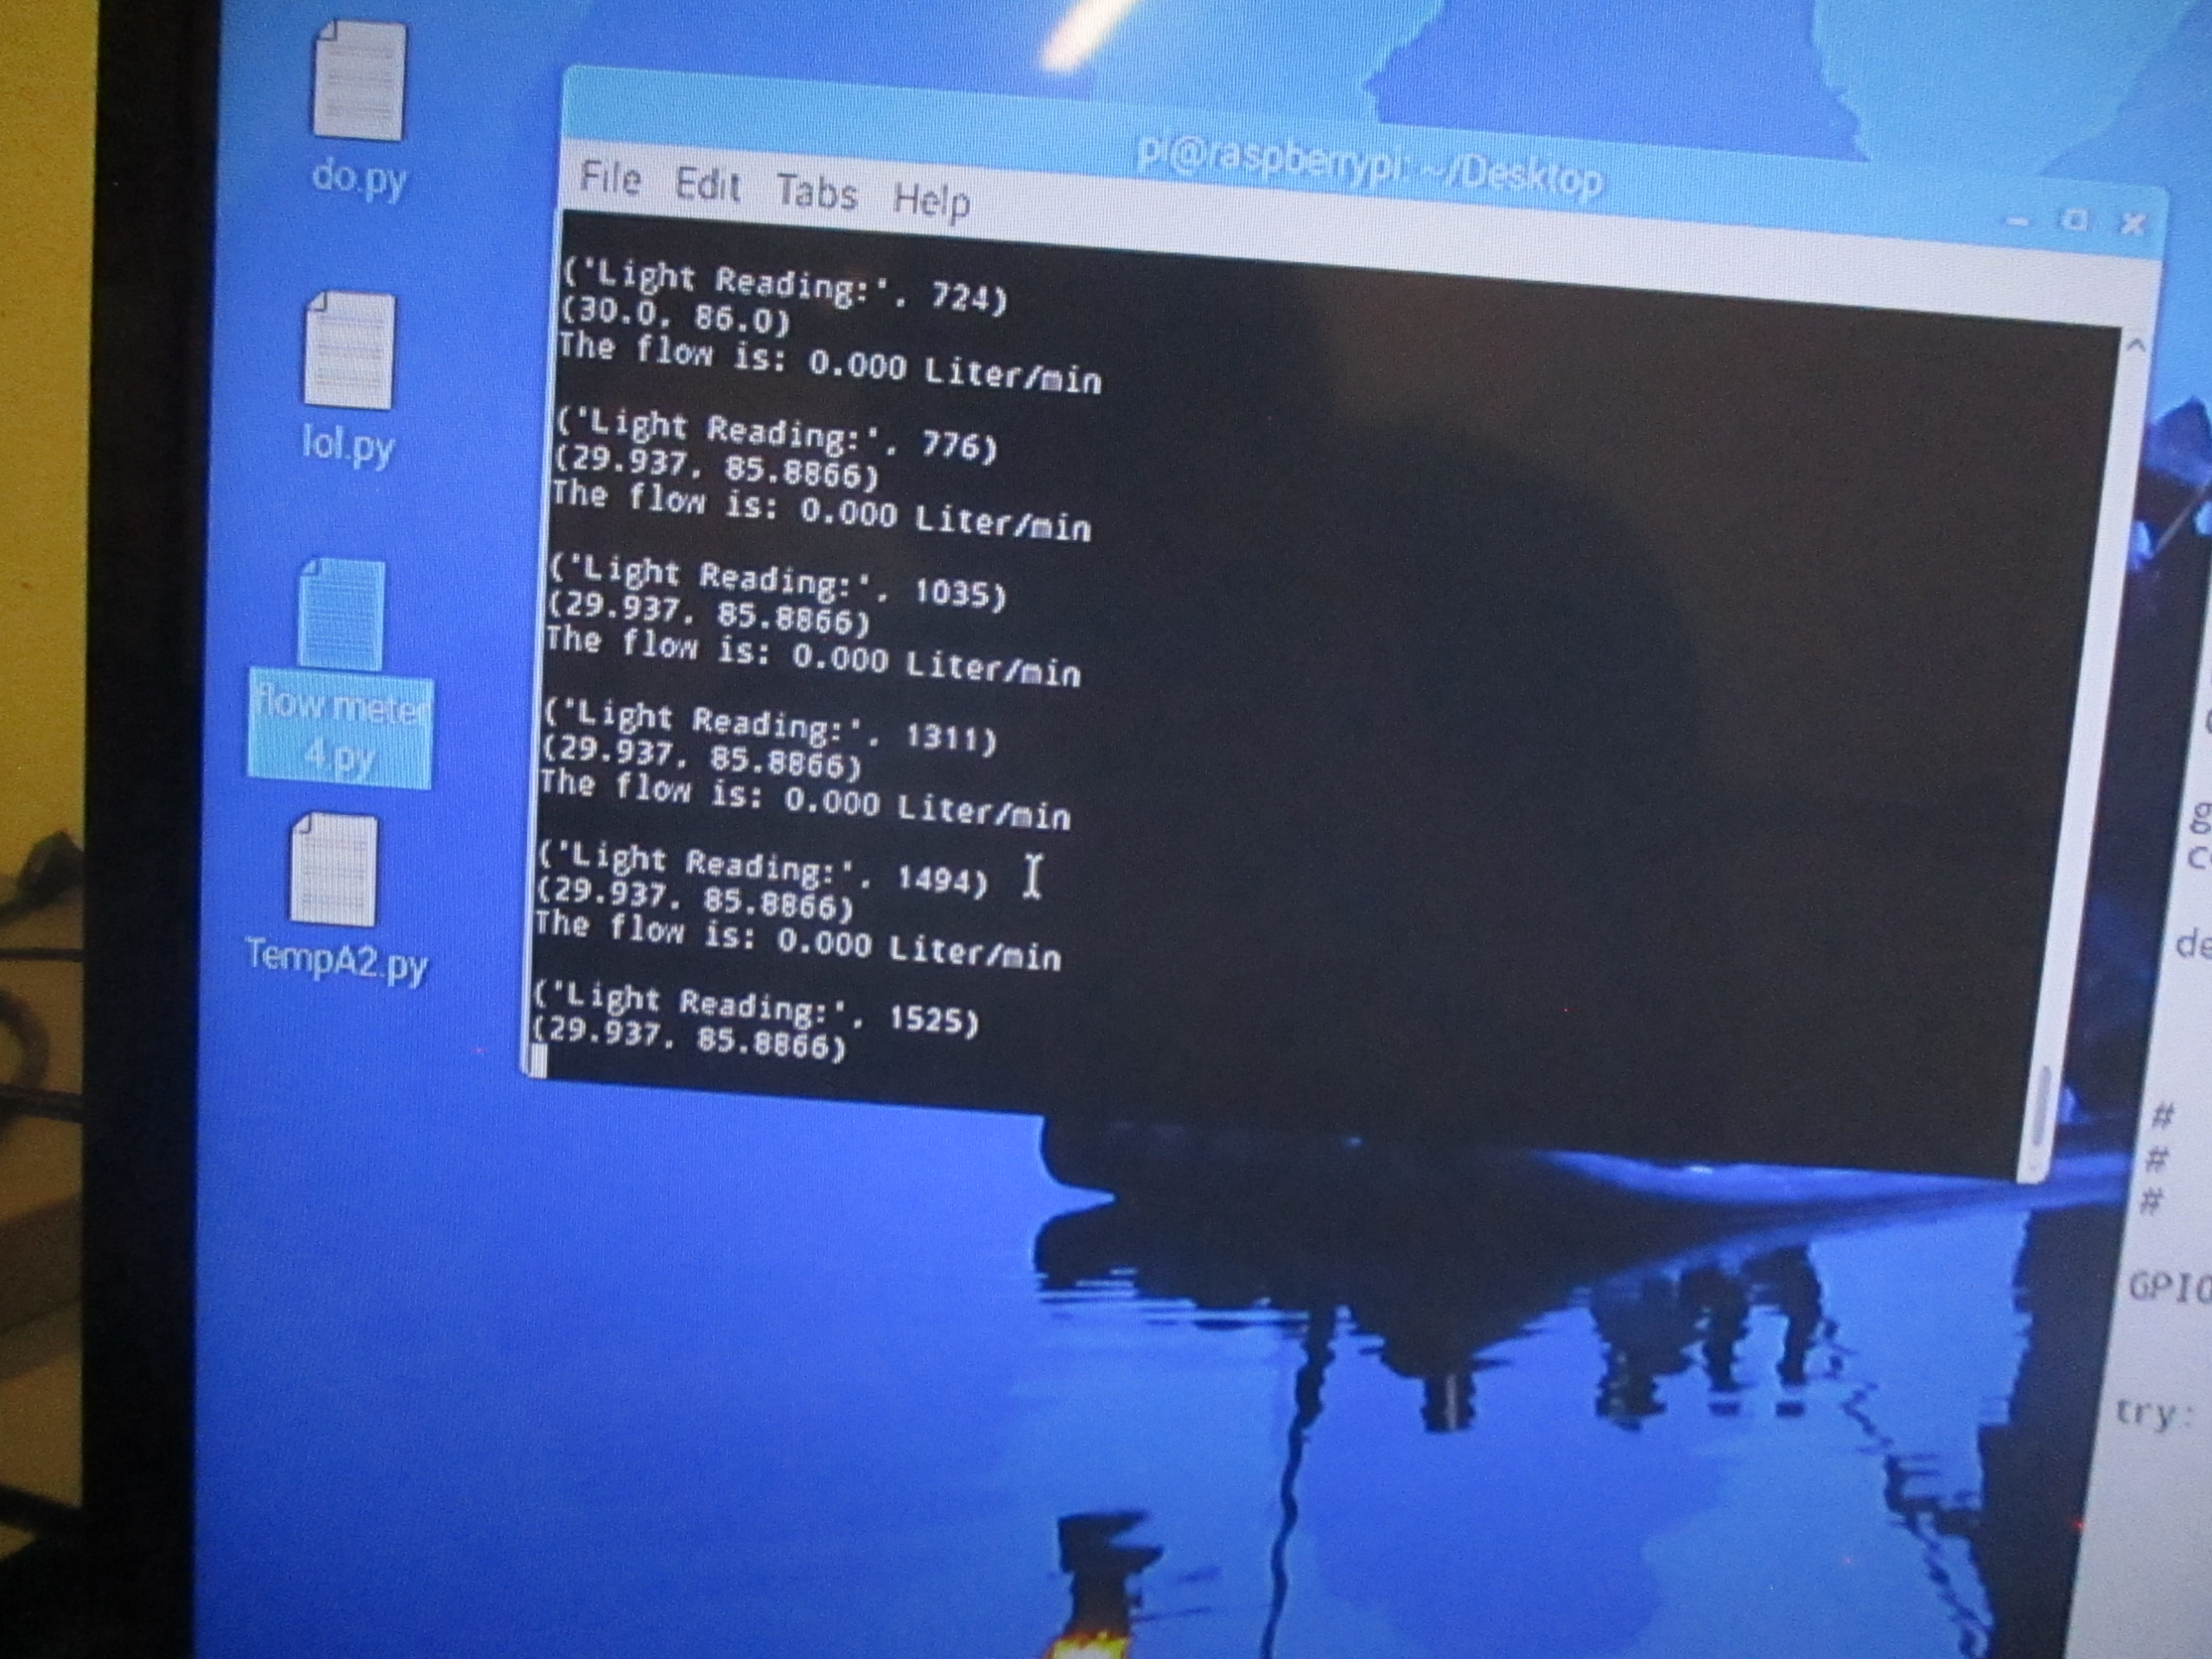
\includegraphics[width=7.5cm]{r4}}
		\subfigure[Riego detenido.]{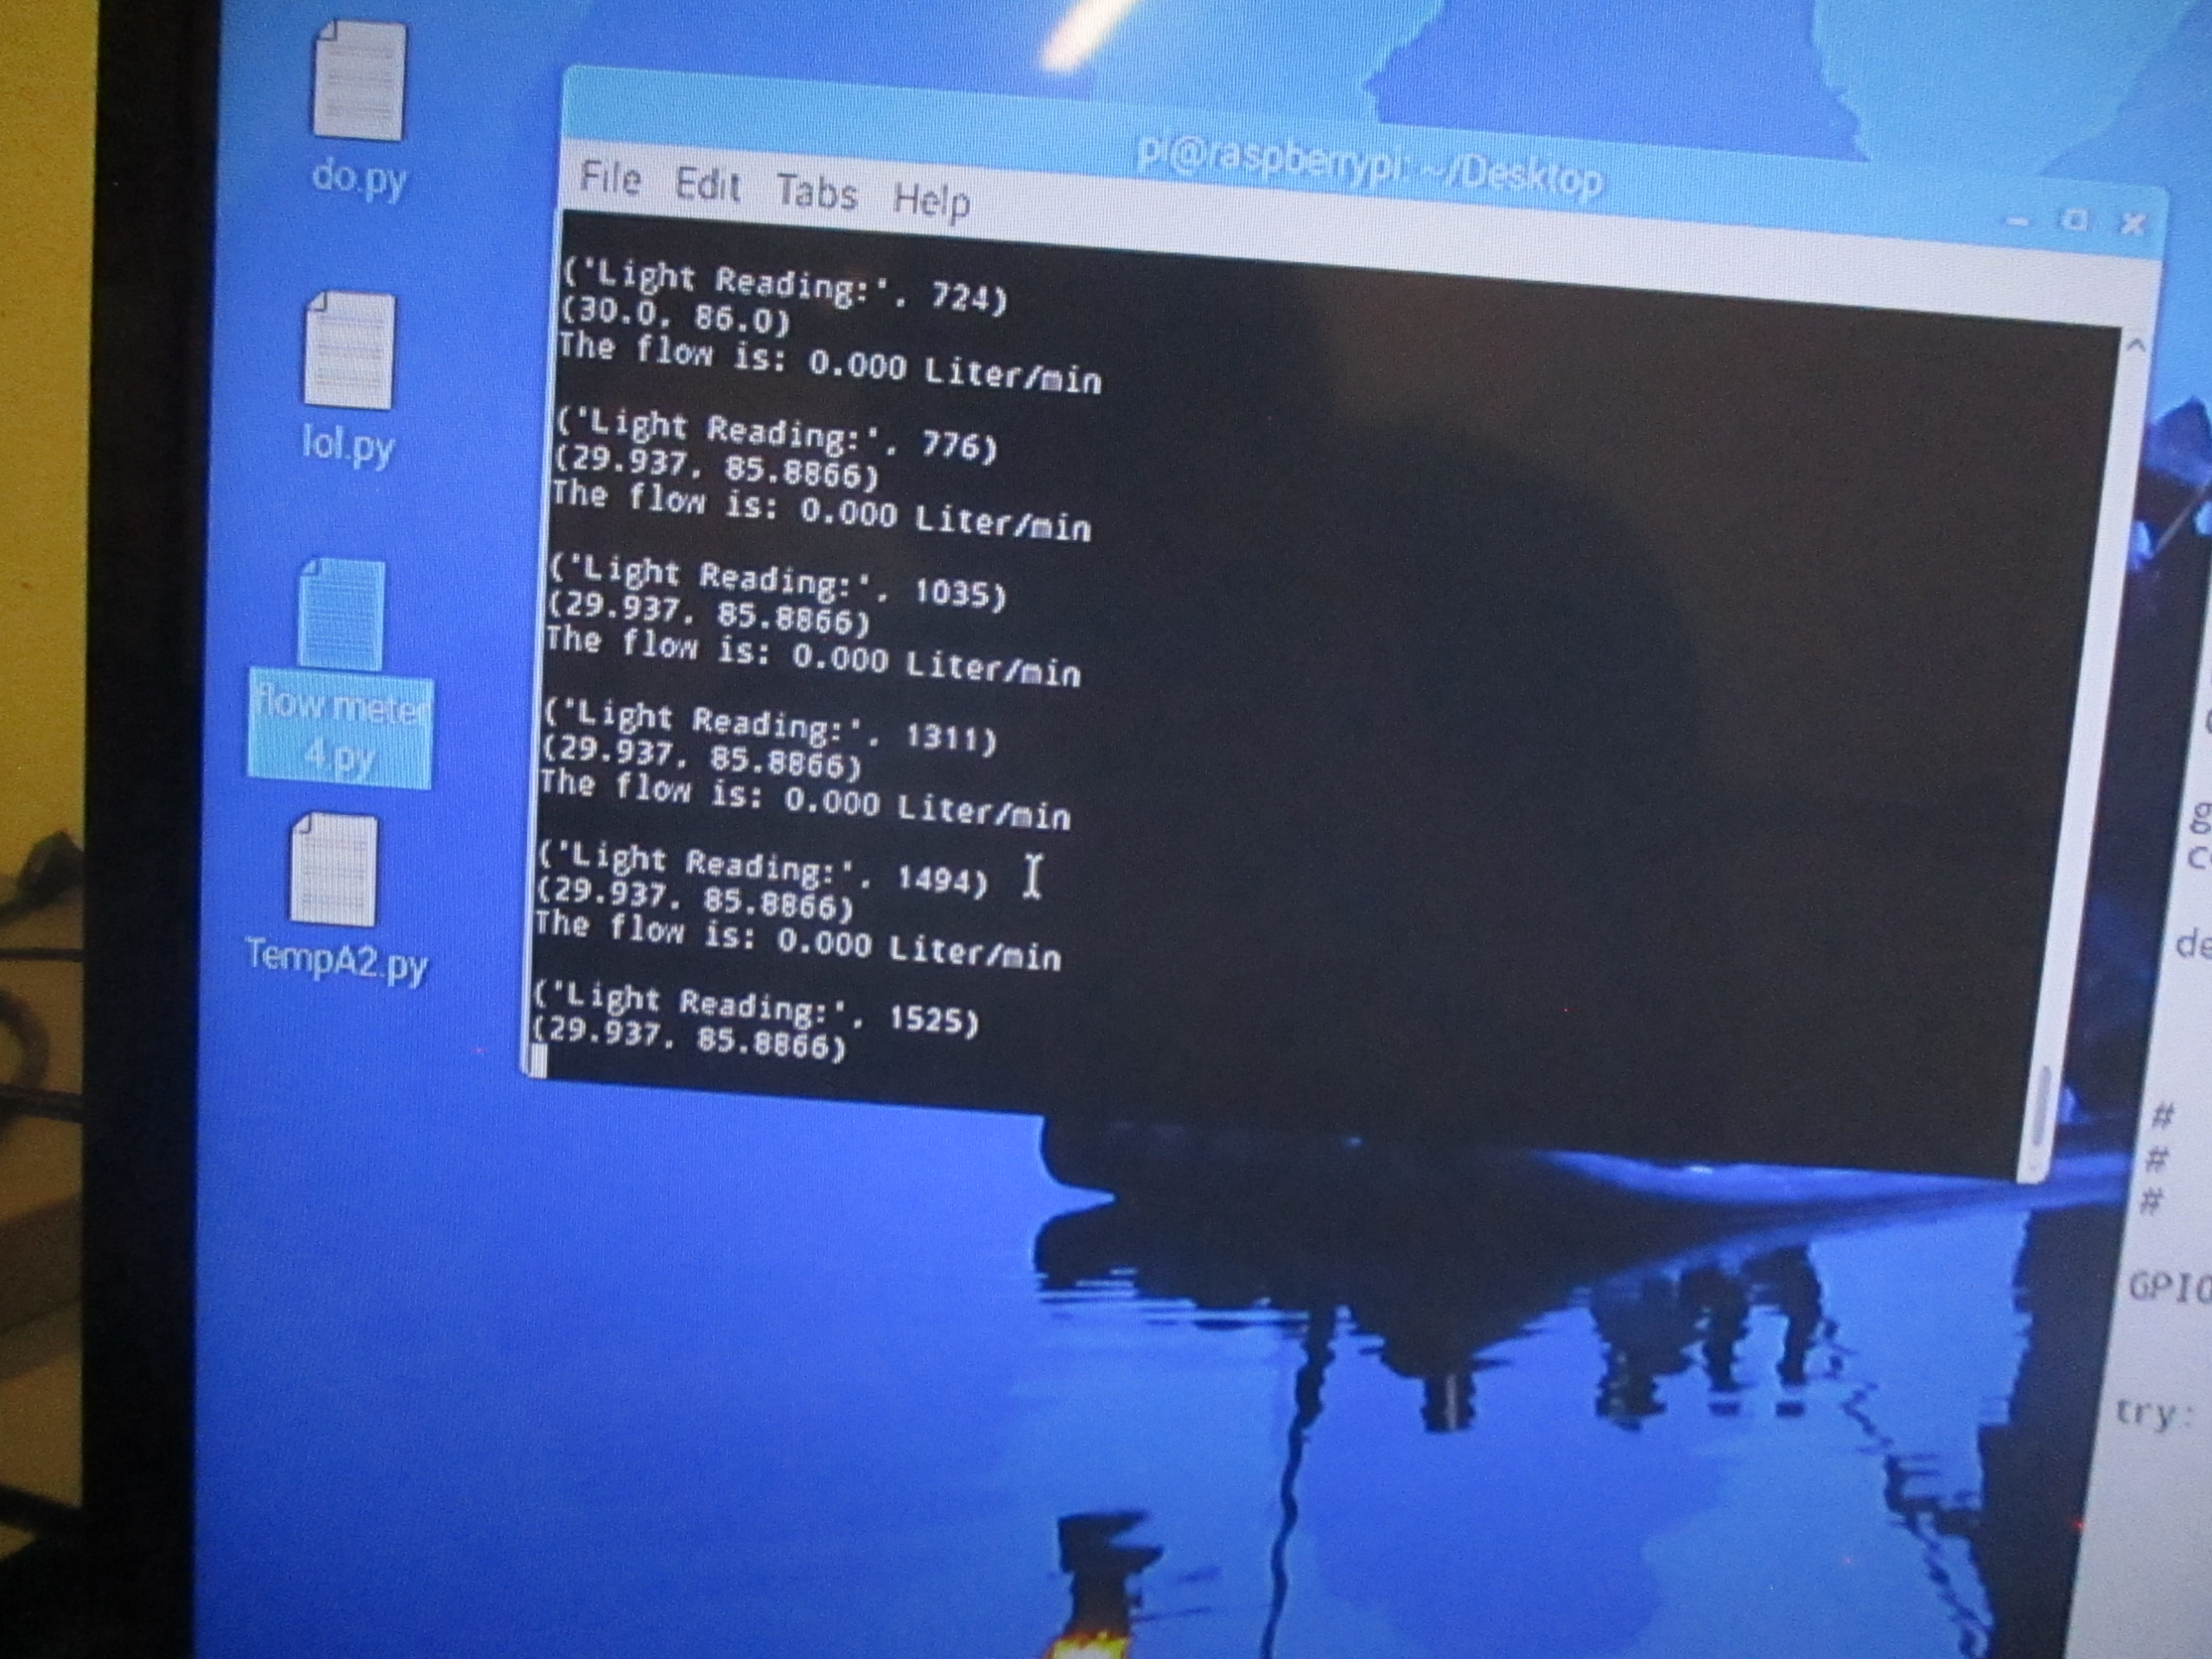
\includegraphics[width=7.5cm]{r4}}
	\end{center}
	\label{evento2}
	\caption{Segundo evento considerado.}
\end{figure} 

Otra forma de detener el flujo de agua, es detectando un nivel de agua bajo parecido al de la imagen \ref{event3}.  

\begin{figure}[H]
	\begin{center}
		\subfigure[Detecci\'on de un bajo nivel de agua.]{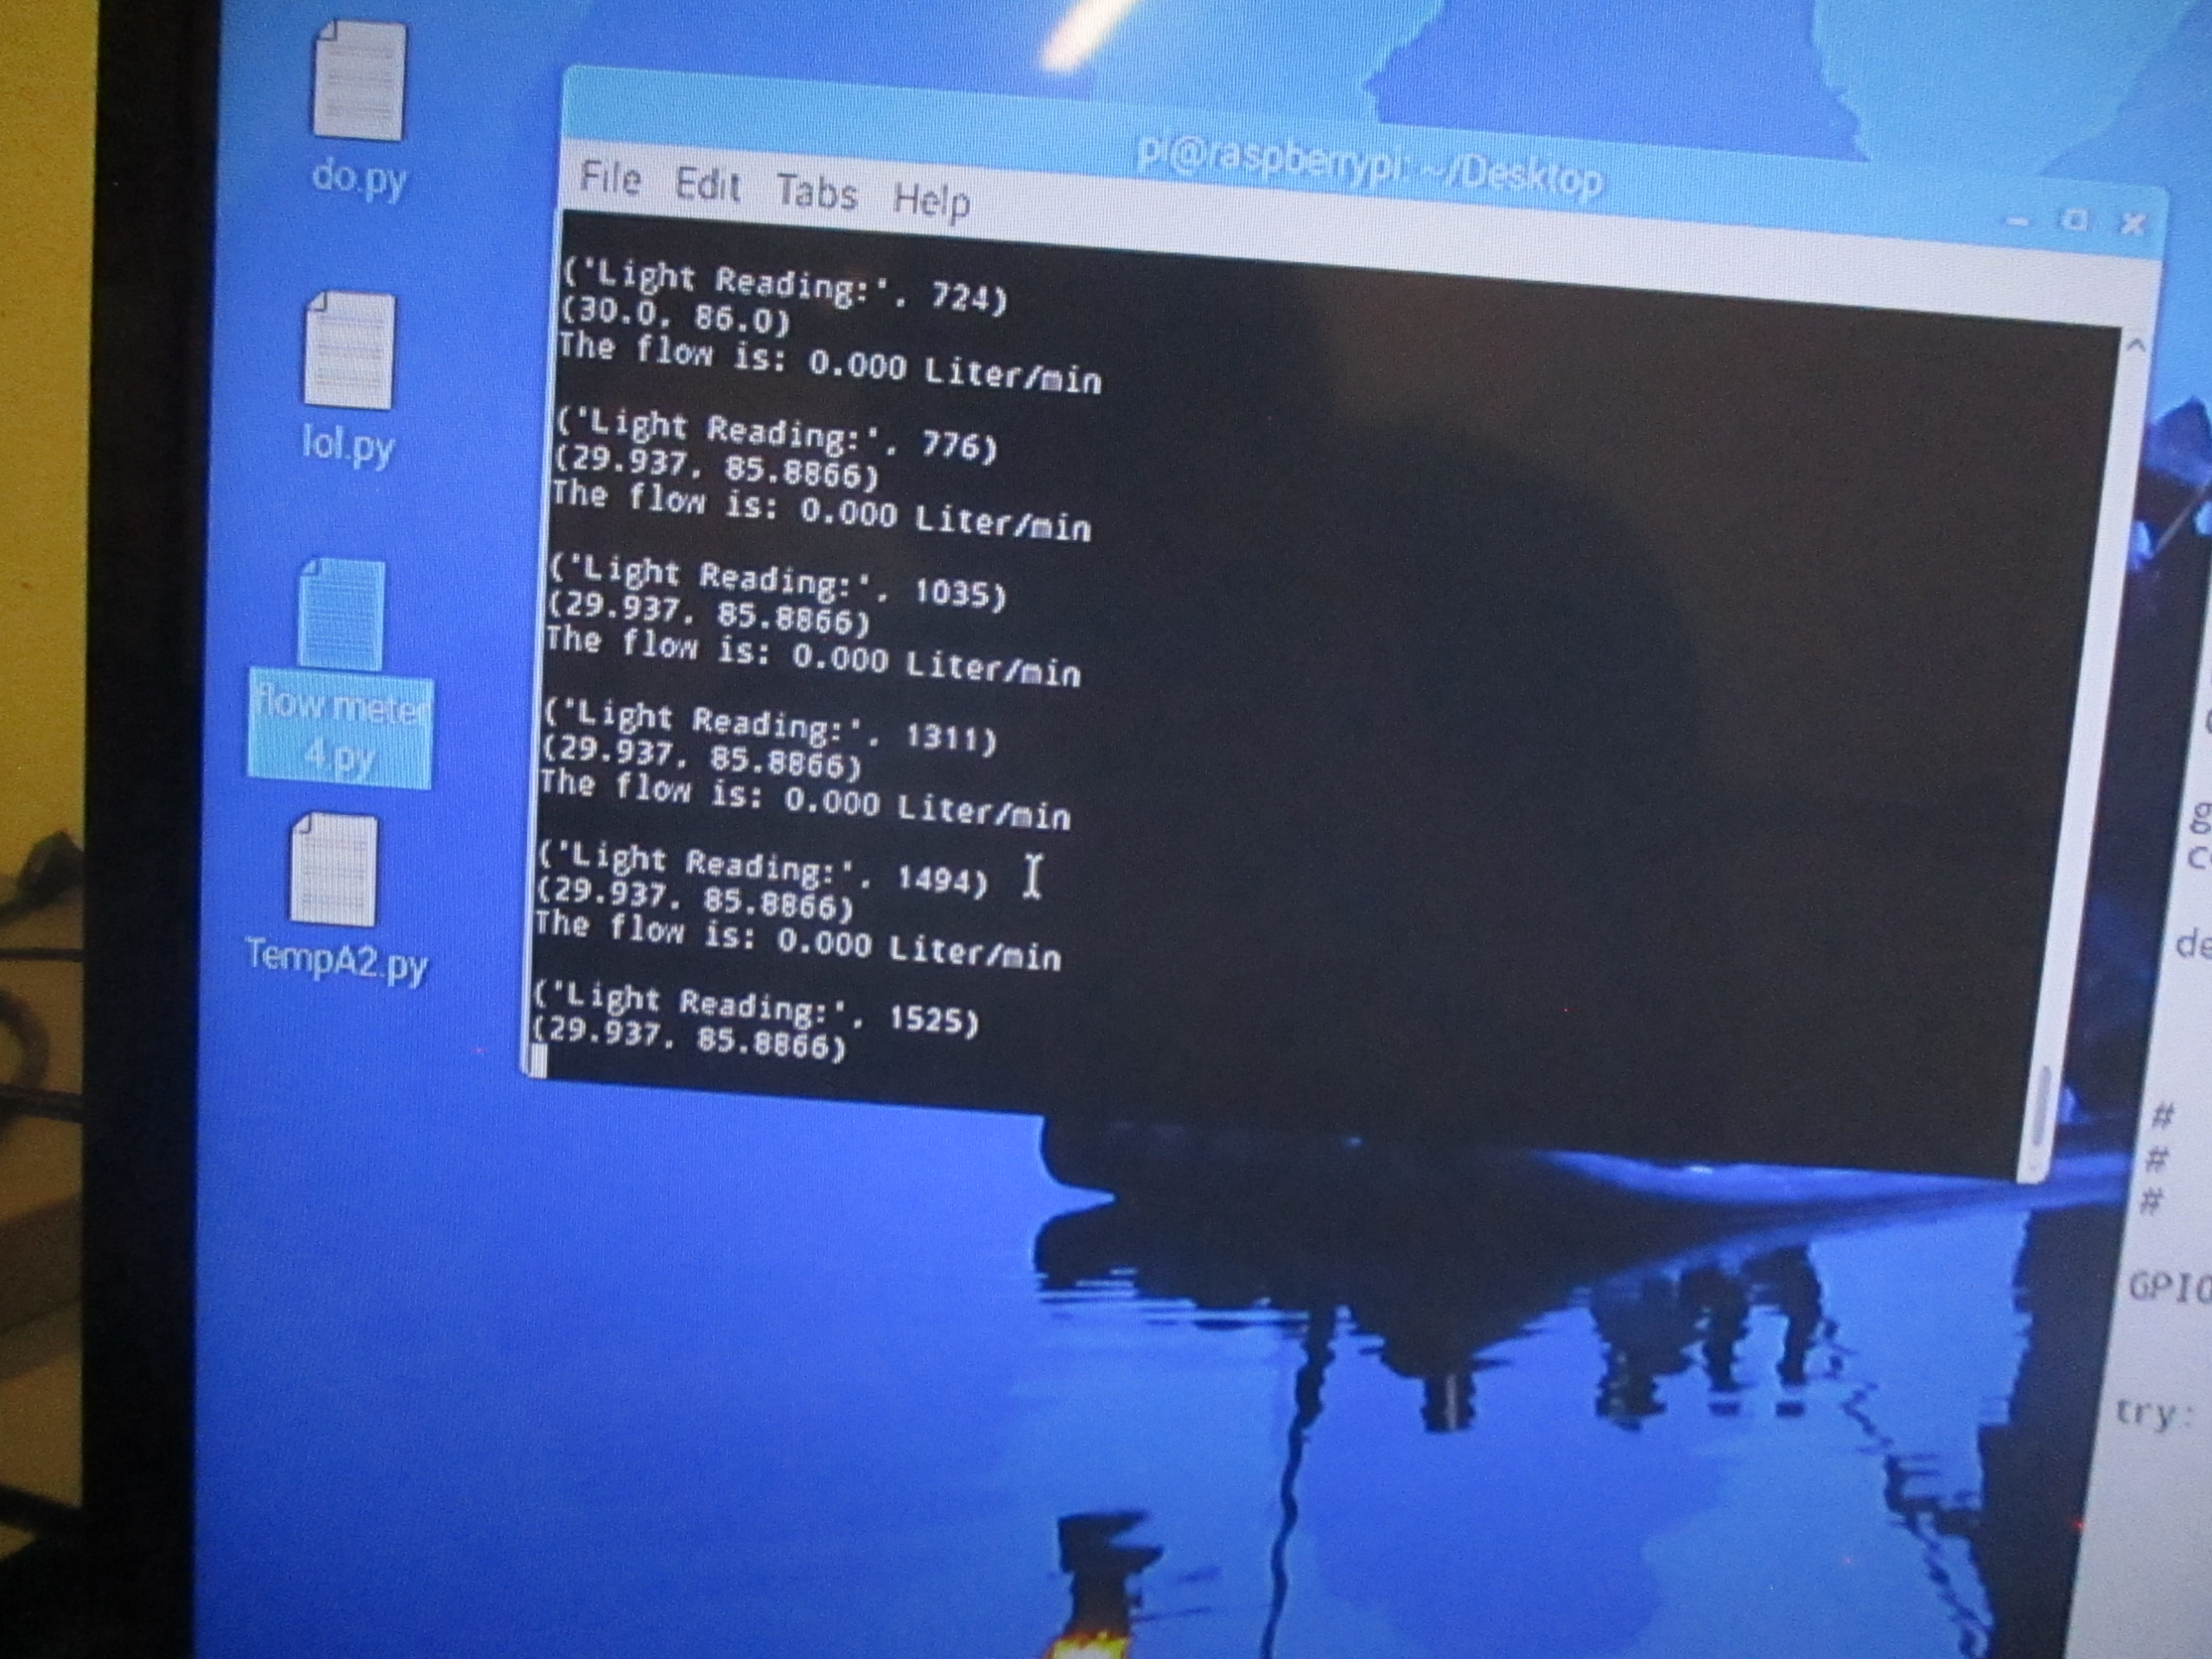
\includegraphics[width=7.5cm]{r4}}
		\subfigure[Riego detenido.]{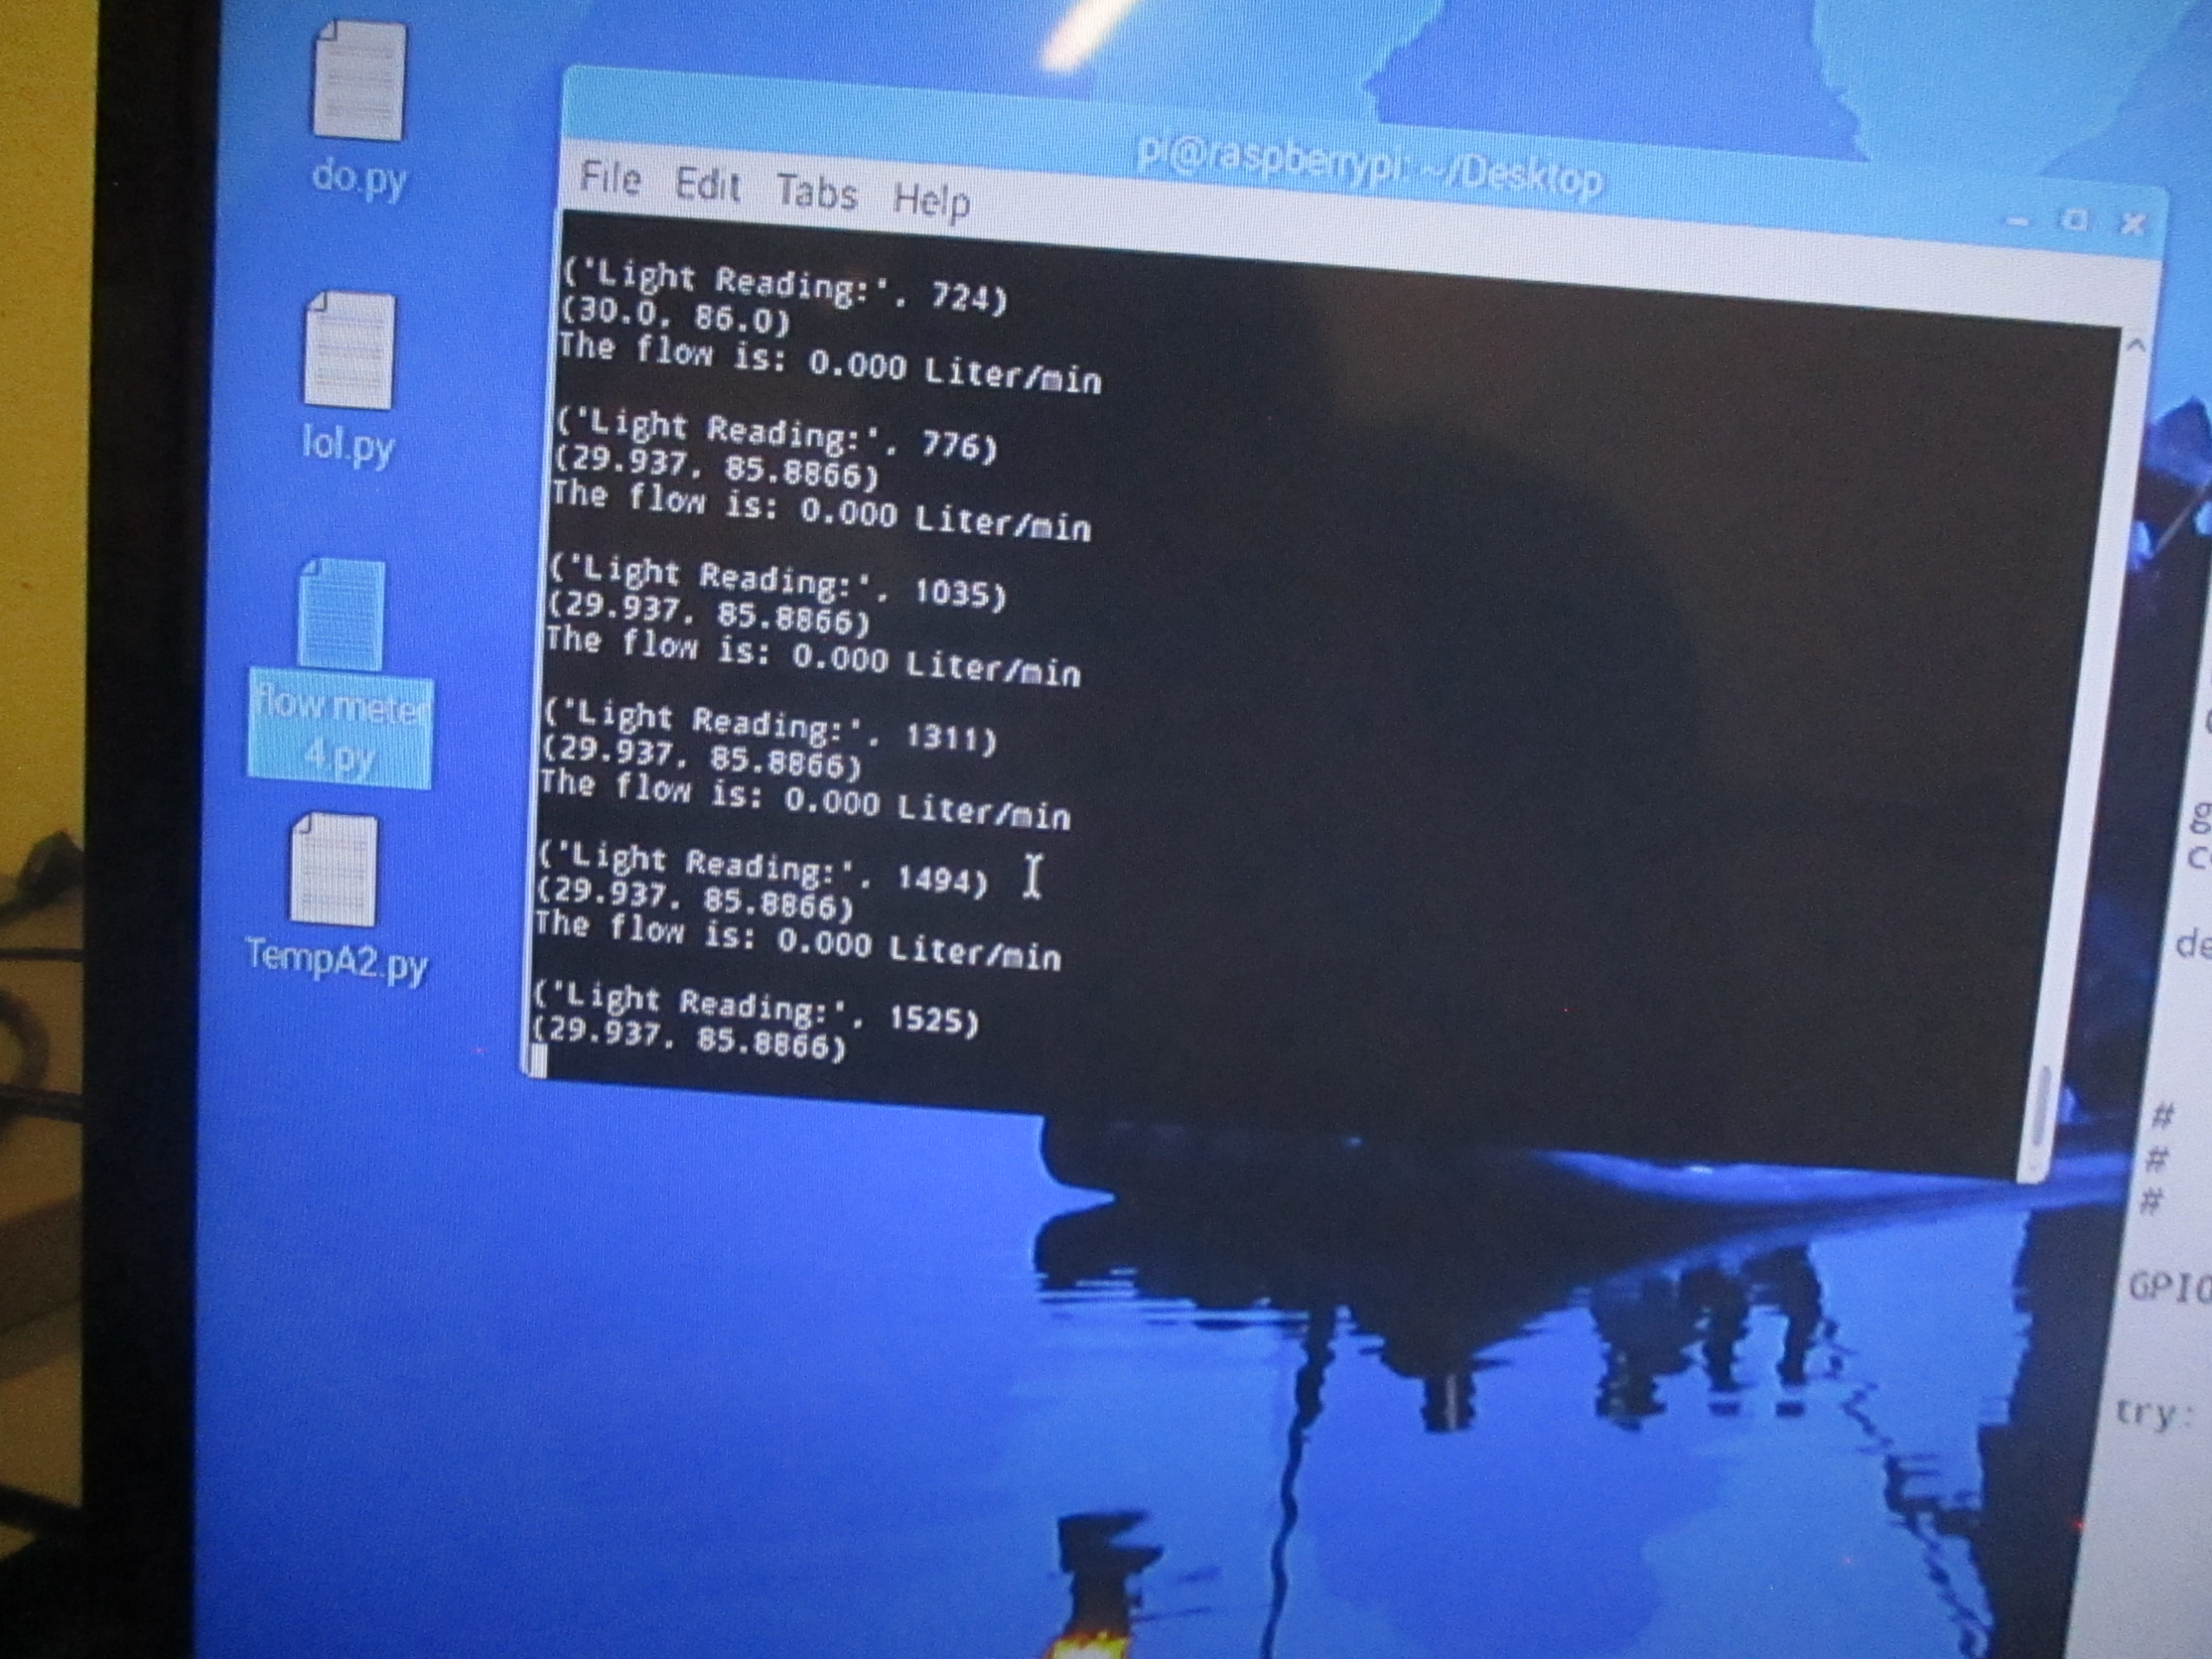
\includegraphics[width=7.5cm]{r4}}
	\end{center}
	\label{event3}
	\caption{Tercer evento considerado.}
\end{figure} 

\end{comment}

\section{Resultados}
El prototipo del sistema de riego super\'o satisfactoriamente las pruebas a las que fue sometido, demostrando as\'i, su eficiencia en cuanto a recopilaci\'on e interpretaci\'on de datos se refiere.\\ 
Como resultado de las pruebas, el prototipo sufri\'o constantes modificaciones de dise\~{n}o tanto en la parte hardware como en la parte de software. En lo que respecta al hardware, todo el sistema cr\'itico fue aislado en una caja, con correspondientes adaptaciones a la misma, y montado sobre un tanque de agua con el resto de los sensores ambientales a su alrededor, tal y como se ve en la imagen 5.4.%\ref{hardwareda}. 

\begin{figure}[H]
	\begin{center}
		\subfigure[Exterior del prototipo.]{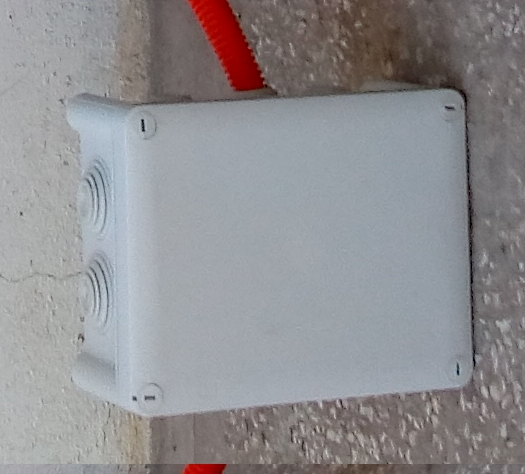
\includegraphics[width=7.5cm]{hardwarec}}
		\subfigure[Interior del prototipo.]{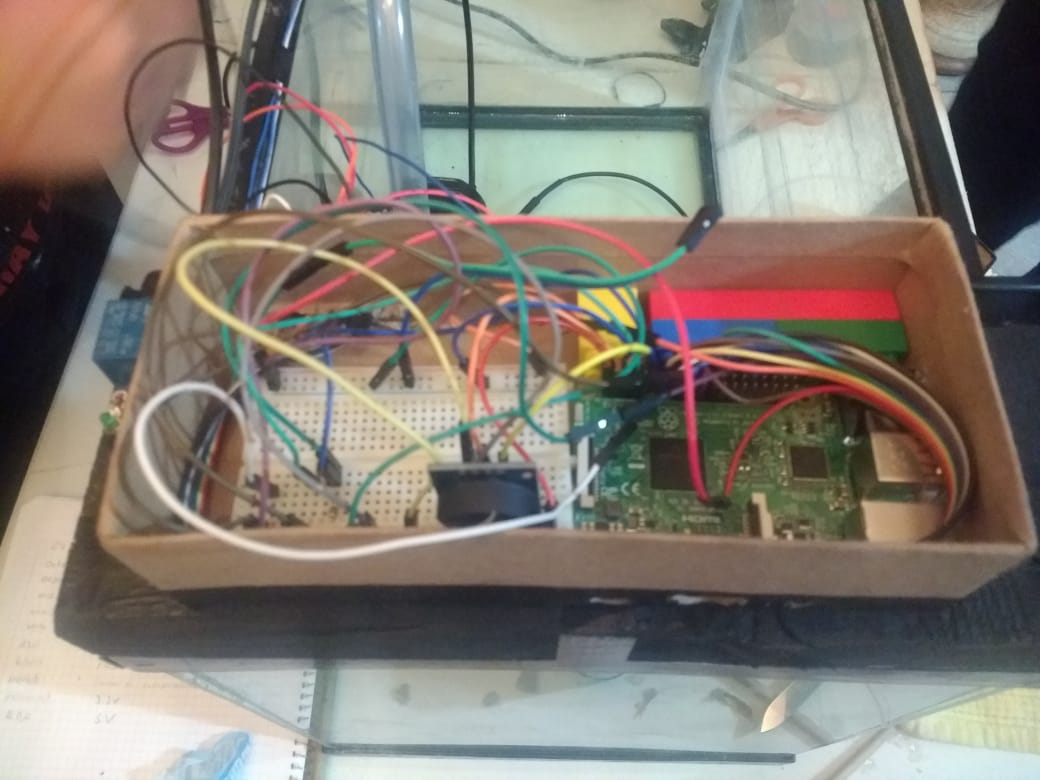
\includegraphics[width=7.5cm]{hardwarea}}
	\end{center}
	\label{hardwareda}
	\caption{Vista del prototipo.}
\end{figure} 

En el caso del software, se desarroll\'o una interfaz gr\'afica simple, de manera que el usuario pueda interactuar con el prototipo de una manera m\'as amigable. La interfaz se puede ver en la imagen \ref{software}.

\begin{figure}[H]
	\begin{center}
		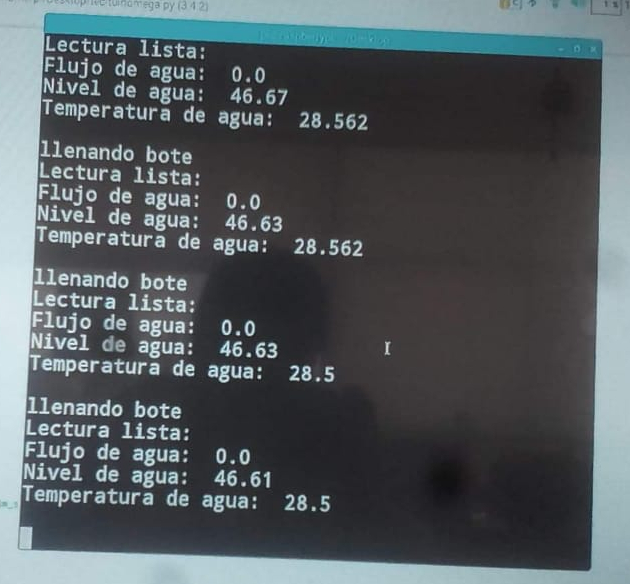
\includegraphics[width=8cm]{software}
	\end{center}
	\caption{Interfaz de usuario del prototipo.}
	\label{software}
\end{figure} 

En la siguiente etapa del proyecto, se reestructur\'o el dise\~no de tal forma que, tanto los sensores utilizados como el funcionamiento del prototipo se visualizaran de forma efectiva. Por otro lado, esto nos ermiti\'o hacer pruebas para analizar dicha actividad. Los sensores conectados se aprecian en la imagen \ref{hardwarep}(a), as\'i mismo, se muestra el sistema en funcionamiento en la \ref{hardwarep}(b).

\begin{figure}[H]
	\begin{center}
		\subfigure[Sensores conectados]{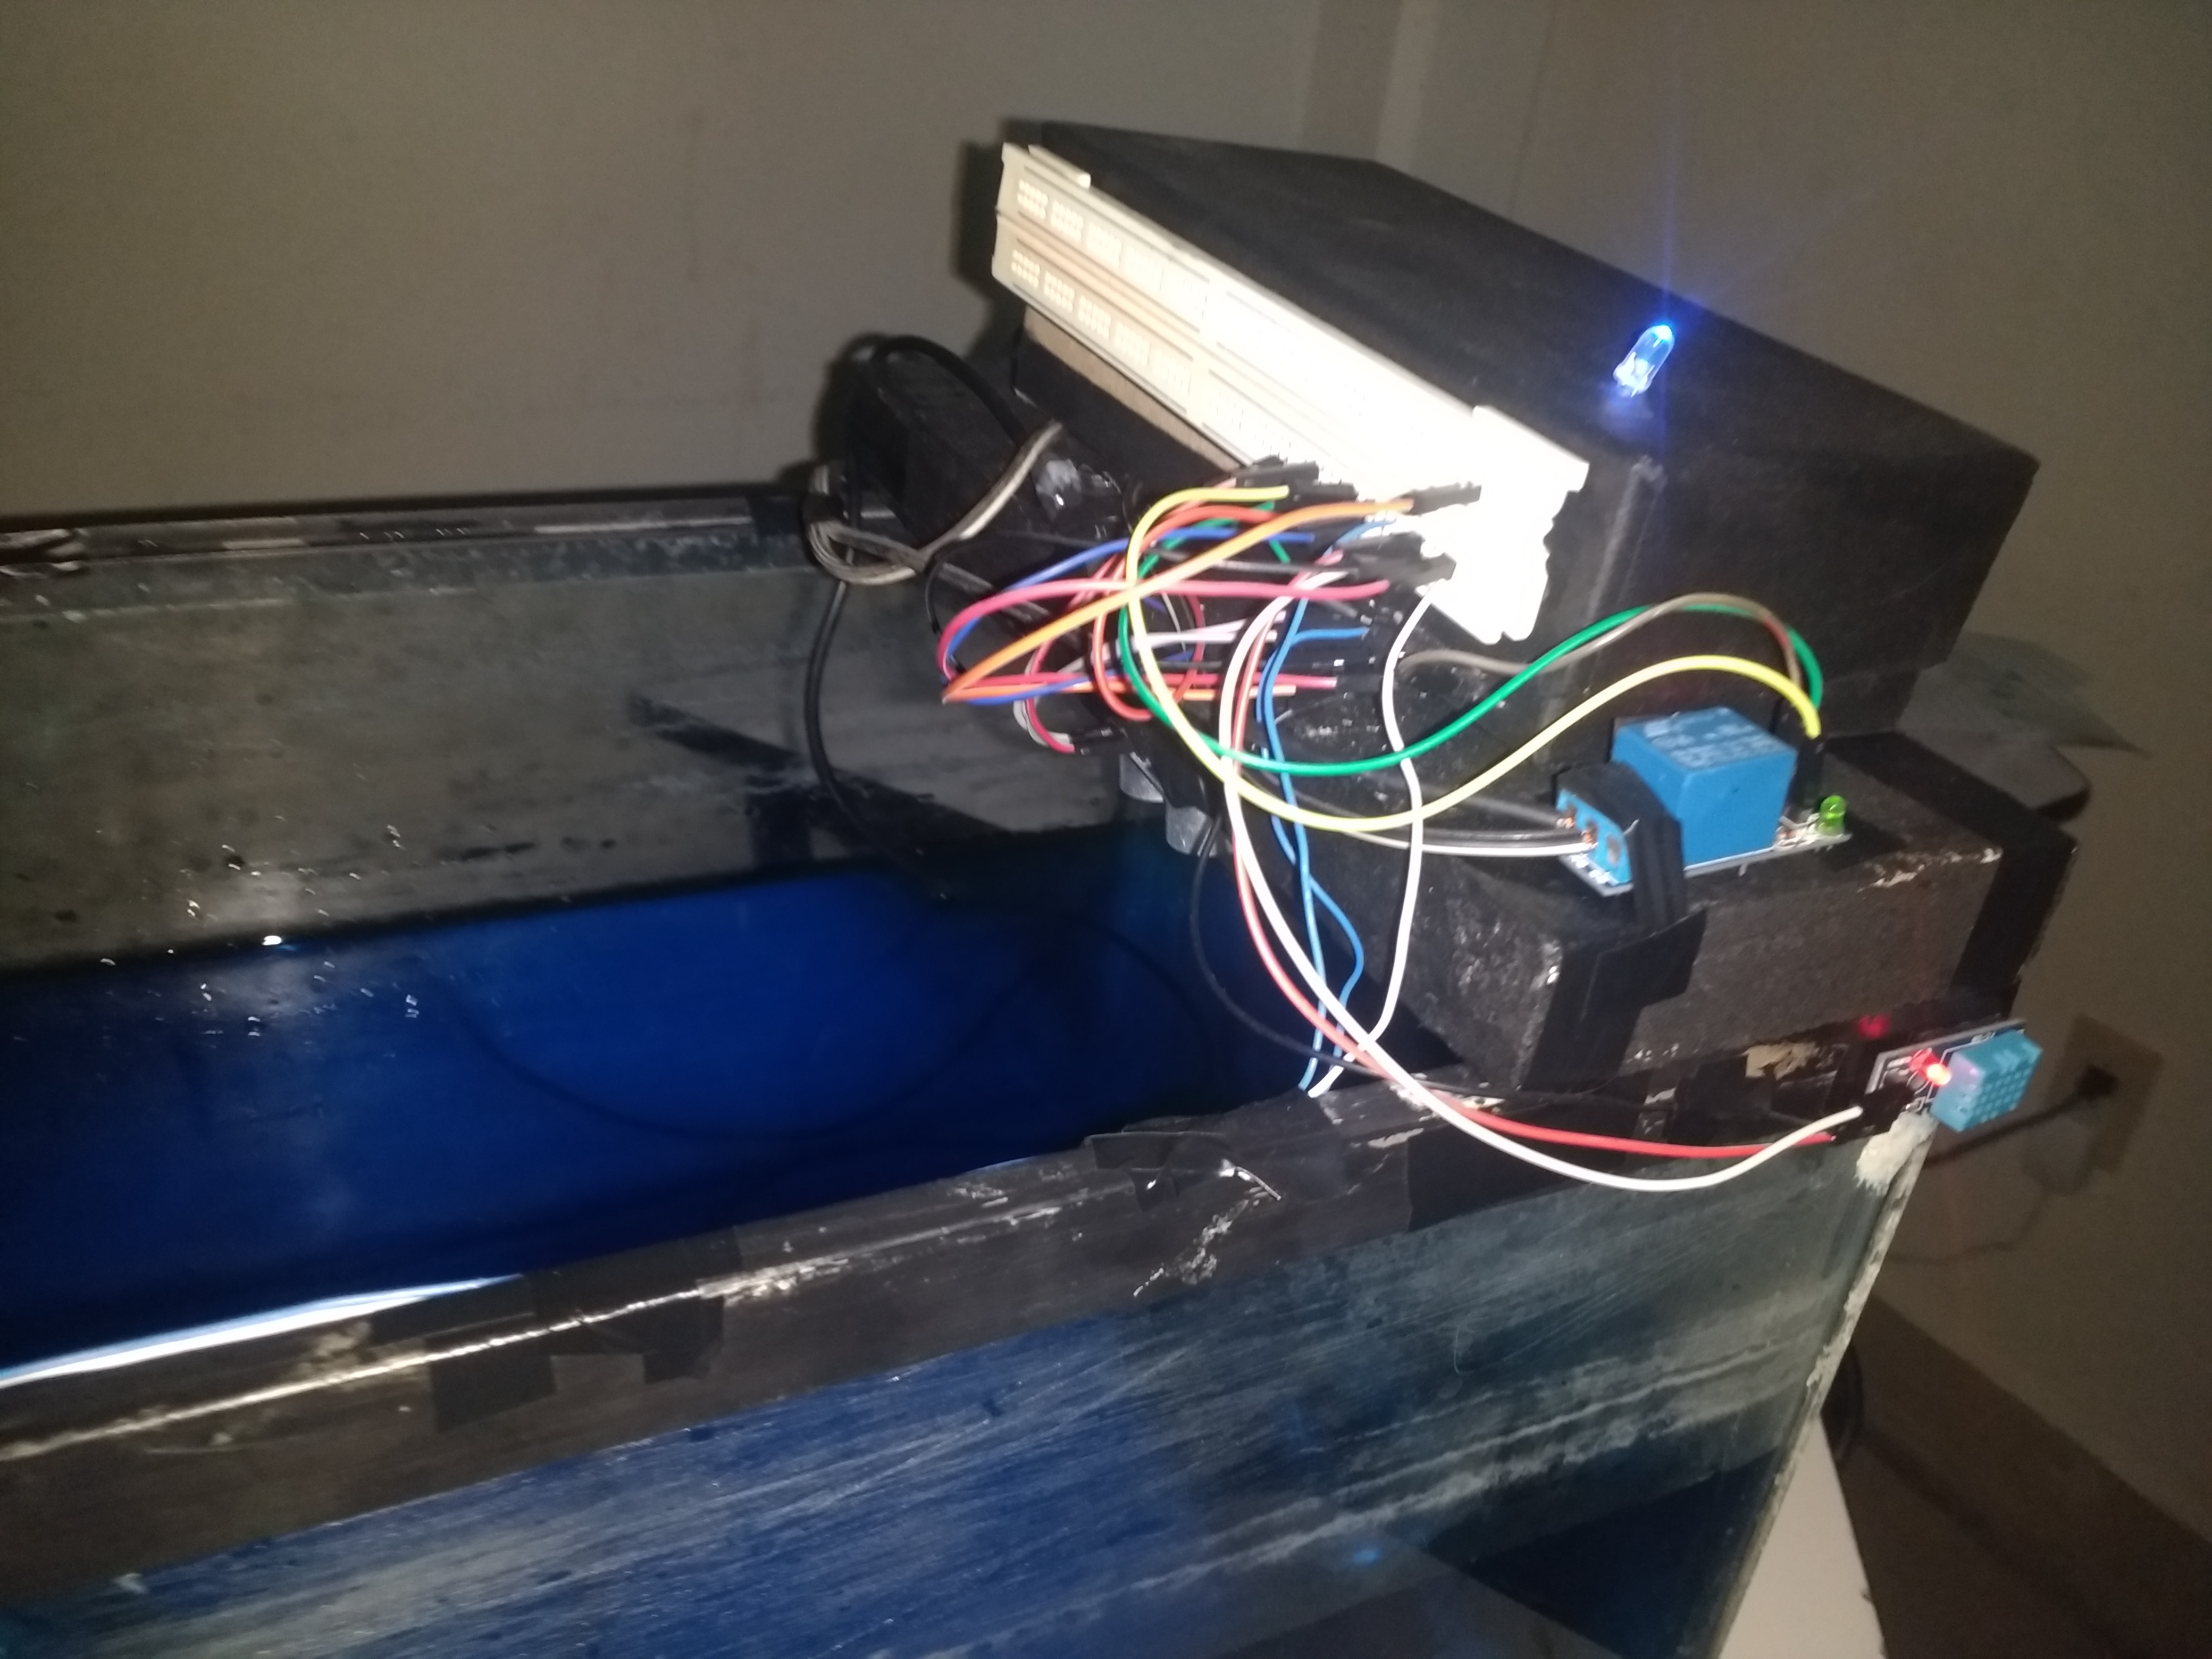
\includegraphics[width=7.5cm]{proto3}}
		\subfigure[Sistema de riego encendido]{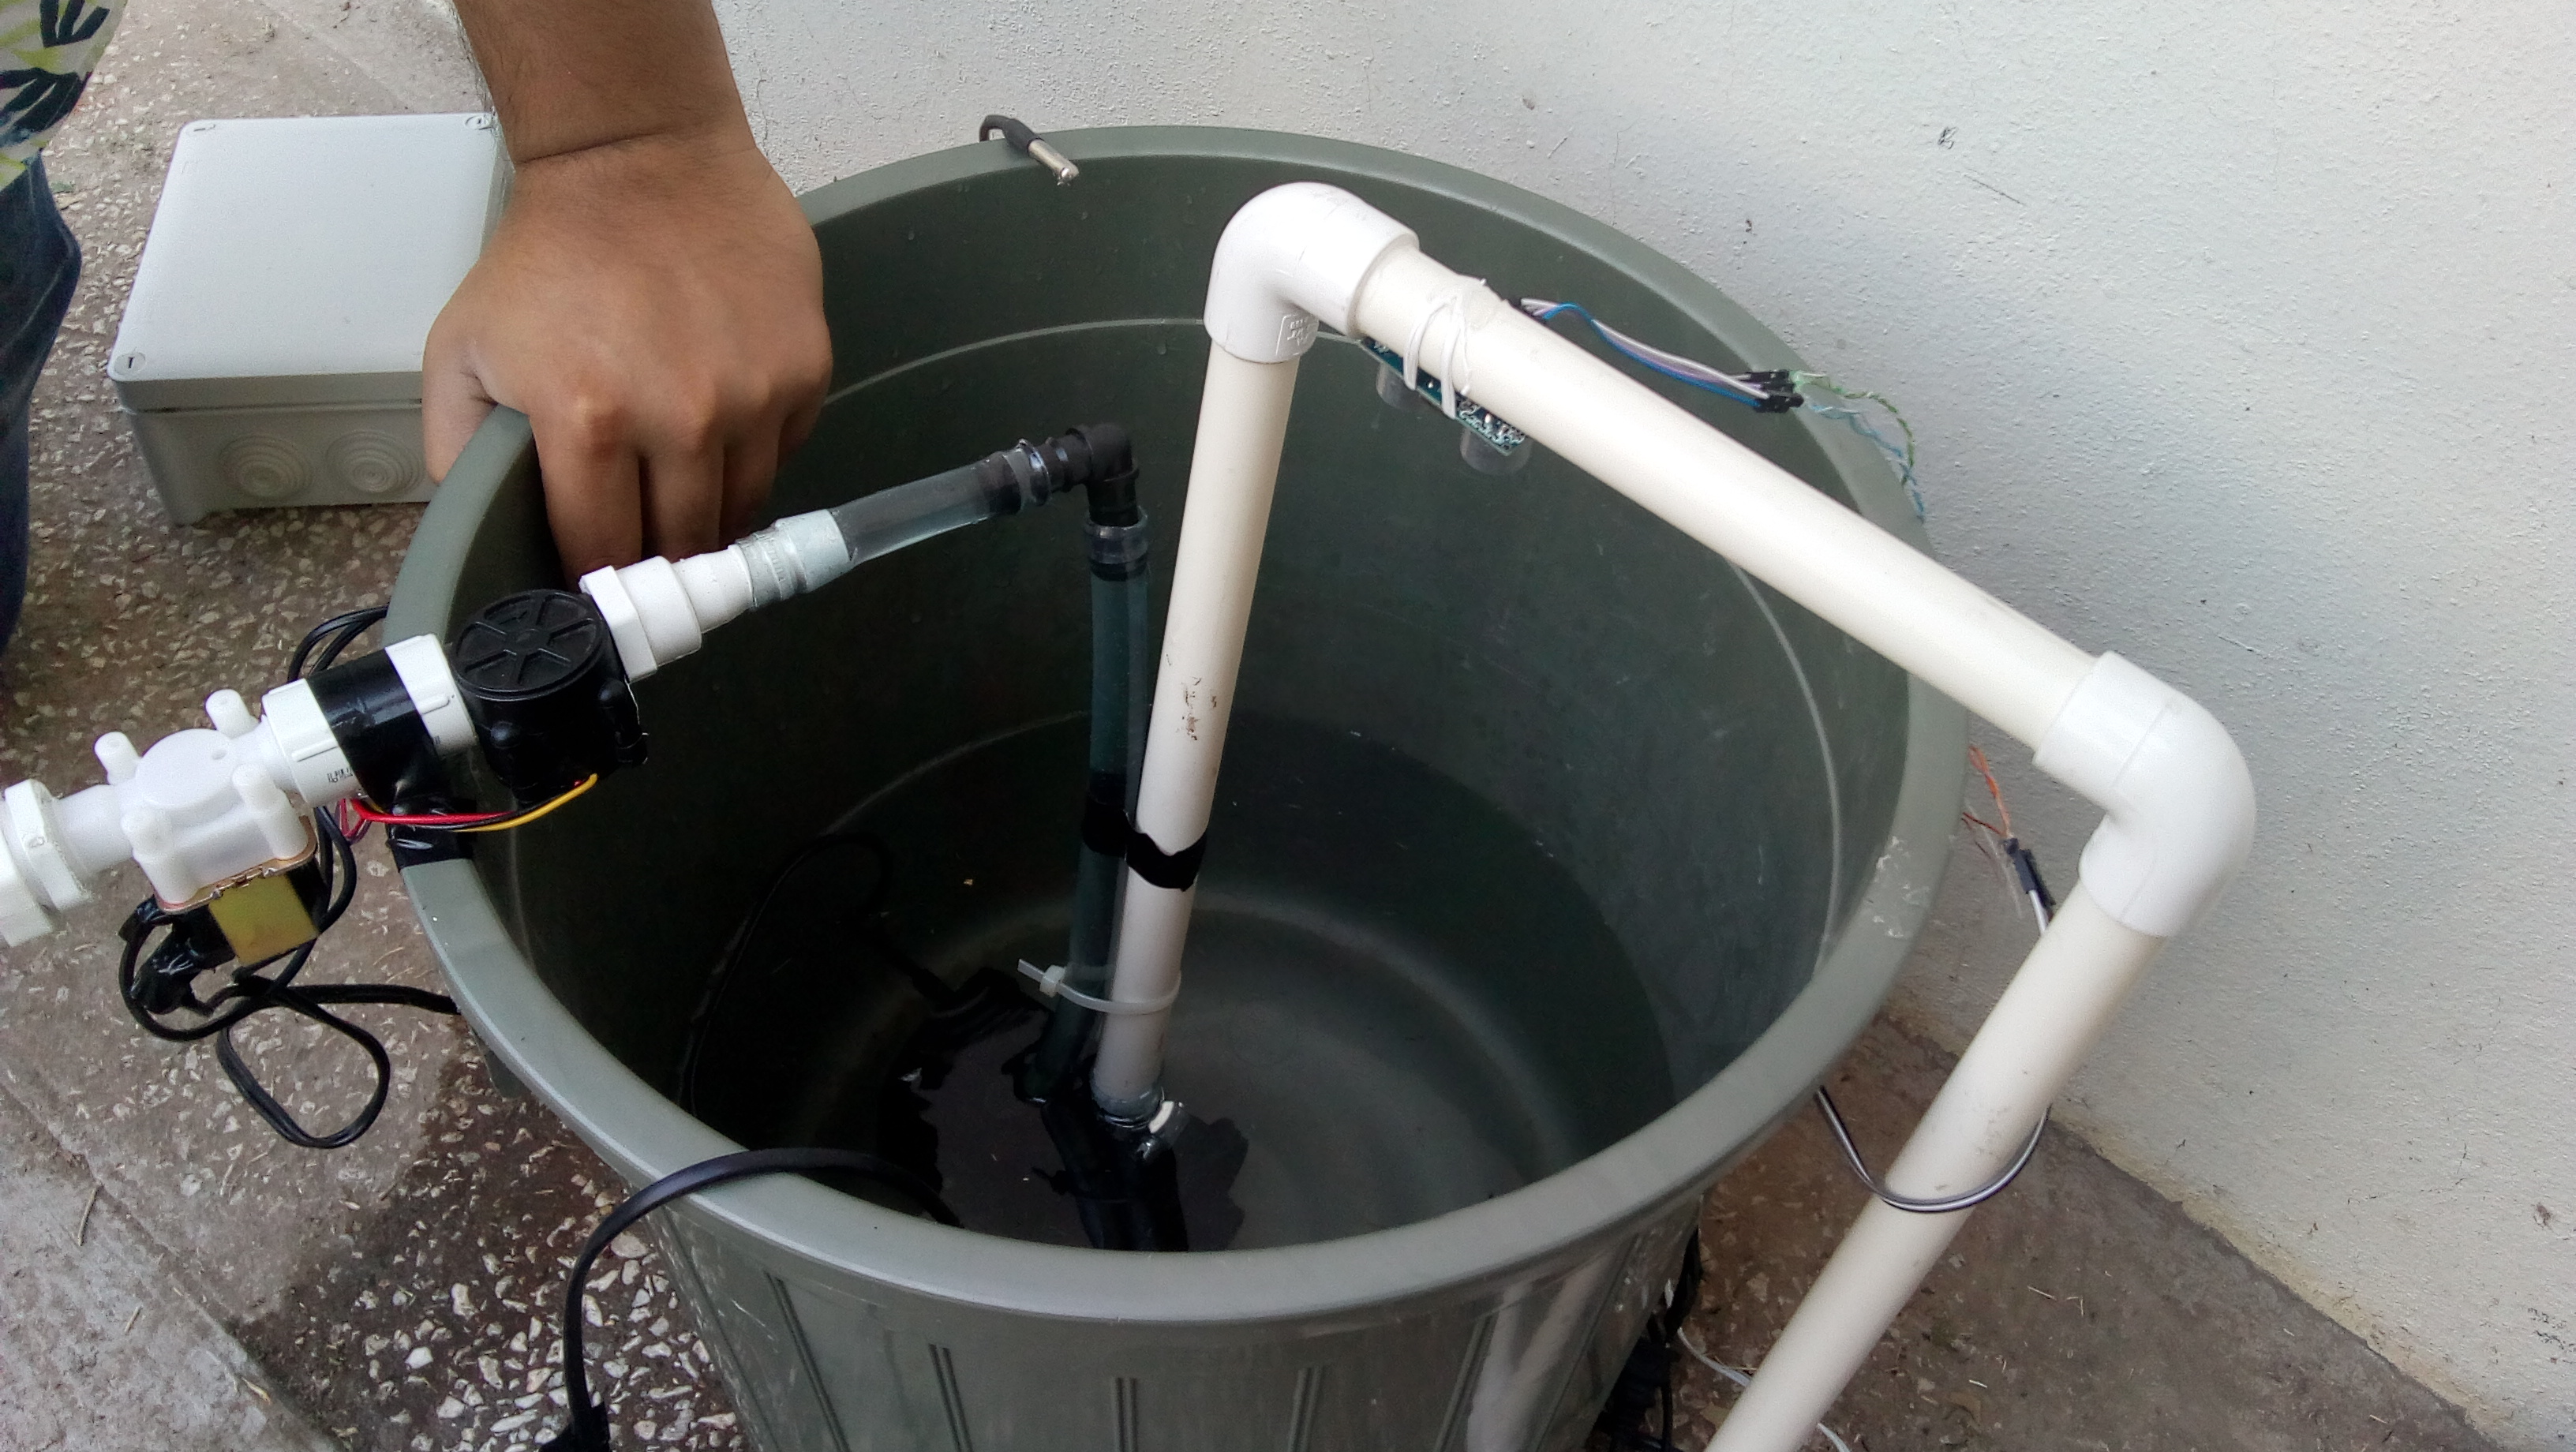
\includegraphics[width=7.5cm]{proto4}}
	\end{center}
	\label{hardwarep}
	\caption{Prototipo funcionando}
\end{figure}

Una parte fundamental del proyecto es la interfaz gr\'afica donde se aprecian los sensores implementados en el prototipo as\'i como los datos que se obtienen de estos sensores, en la imagen \ref{interfaz} se muestra la interfaz desarrollada para el prototipo.
\begin{figure}[H]
	\begin{center}
		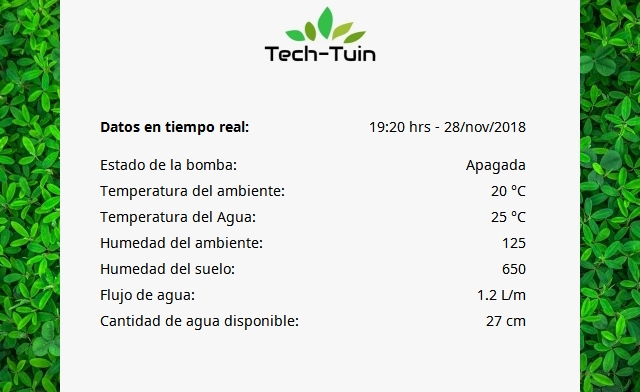
\includegraphics[width=13cm]{Interface}
	\end{center}
	\caption{Reestructuraci\'on de Interfaz gr\'afica.}
	\label{interfaz}
\end{figure} 
\newpage
%\chapter{Conclusiones}

\begin{thebibliography}{X}
	\bibitem{1} Tejada, Marcia (2013). Jarduino, Sistema de riego manejado por Arduino (Documento in�dito). Seminario: Introducci�n a la programaci�n de microcontroladores con tecnolog�as libres. UNQ.
	\bibitem{2} Gil-Albert V. F,(2006),Manual t�cnico de jardiner�a I. Establecimiento de jardines, parques y espacios verdes, Madrid Espa�a, Mundi-prensa.
	\bibitem{3} Torrecilla C.M,(1998),Manual practico de la jardiner�a, Madrid Espa�a,EL PA�S.
	\bibitem{4} Daniel Rios Cruellas. (2016). Sistema de riego autom�tico. 2016, de universitat polit�cnica de catalunya Sitio web: https://upcommons.upc.edu/handle/2117/105385
	\bibitem{5} Fernando Escamilla Mart�nez . (2016). AUTOMATIZACI�N Y TELECONTROL	DE SISTEMAS DE RIEGO. febrero,20,2016, de UNIVERSIDAD POLITECNICA DE VALENCIA.
	\bibitem{6} Gabriel Escalas Rodr�guez . (2014). Dise�o y desarrollo de un prototipo de riego autom�tico controlado con Raspberry Pi y Arduino Y TELECONTROL DE SISTEMAS DE RIEGO. febrero,6,2014, de Universidad politenica de catalunya Sitio web:https://upcommons.upc.edu/bitstream/handle/2099.1/25074/
	memoria.pdf?sequence=4\&isAllowed=y
	\bibitem{7} Armando Torrente Trujillo ,Iv�n Dar�o M�ndez G , Edward Iv�n L�pez R. . (2015). Dise~no de un sistema de riego por microaspersi�n automatizado para el cultivo de guan�bana mediante el uso de las herramientas SIG. Agosto,6,2014, de Universidad Surcolombiana Neiva
	
	\bibitem{8} Mart�n Tarjuelo. (2010). El riego y su tecnolog�a. M�xico: Mundi-Prensa
	\bibitem{9} Francisco Miguel �guila Mar�n. (2008). Agricultura T�cnica en M�xico. M�xico: Universidad
	Hohenheim.
	\bibitem{10} Yessica S�ez. (2017). Sistema de Riego Inteligente para Optimizar el Consumo de	Agua. Panam�: Universidad Tecnol�gica de Panam�.
	\bibitem{11}  Comisi�n estatal del agua (2007). Gu�a de ahorro y reutilizaci�n del agua. Guanajuato, p.12.
\end{thebibliography}
\end{doublespace}
%\newpage
%\bibliographystyle{plain}
%\nocite{*}
%\bibliography{Tesis}

\end{document}
